\chapter{Release 1 : Cœur applicatif}

\section{Introduction}

La Release 0 a livré le socle technique de la plateforme : cluster Kubernetes isolé par tenant, exécution serverless via Knative Serving, bus d'événements Kafka opéré par Strimzi. La Release 1, objet de ce chapitre, organise le cœur applicatif de la plateforme par domaine de gestion fonctionnelle, plutôt que par brique technique livrée : chaque sprint regroupe l'ensemble des fonctionnalités d'un même domaine, tous les acteurs concernés confondus, et livre conjointement la brique backend et l'écran du portail qui l'expose.

Elle regroupe quatre sprints : le Sprint 3, qui met en place les accès et l'identité des utilisateurs, préalable à tout le reste ; le Sprint 4, qui livre le cycle de vie complet d'une application ; le Sprint 5, qui relie Kafka et Knative Eventing en un service de messagerie événementielle complet, de la brique backend jusqu'aux écrans du portail ; et le Sprint 6, qui livre l'observabilité applicative (journaux, métriques).

\clearpage
\section{Sprint 3 : Gestion des utilisateurs et des accès}

\subsection{Introduction}

Ce sprint met en place l'identité et le contrôle d'accès de la plateforme : création de compte, connexion, gestion du profil, gestion des rôles côté ADMIN, gestion d'équipe côté CLIENT\_ADMIN. Aucune autre fonctionnalité de la plateforme ne peut être protégée par rôle ou par permission tant que ce socle n'existe pas ; ce sprint précède donc logiquement tous les suivants.

L'authentification passe entièrement par Keycloak. Le backend ne gère ni mot de passe ni session : c'est un serveur de ressources OAuth2, qui valide les jetons émis par Keycloak et en extrait le rôle applicatif.

\subsection{Sprint Backlog}

Le tableau~\ref{tab:sb-sprint3} présente le backlog détaillé du Sprint 3, obtenu en décomposant chaque User Story retenue en tâches techniques.

\needspace{0.9\textheight}
{
\setlength{\LTleft}{-1.5cm}
\setlength{\LTright}{-1.5cm}
\setlength{\tabcolsep}{8pt}
\renewcommand{\arraystretch}{1.9}
\begin{longtable}{|p{6.6cm}|>{\raggedright\arraybackslash}p{8.1cm}|>{\centering\arraybackslash}p{2.3cm}|}
\hline
User Story & Tâches & Estimation \\
\hline
\endfirsthead
\hline
User Story & Tâches & Estimation \\
\hline
\endhead
\hline
\endfoot

\caption{Backlog du Sprint 3}
\label{tab:sb-sprint3}
\endlastfoot

\multirow{3}{6.6cm}{\centering En tant que CLIENT\_ADMIN, je veux créer un compte afin d'accéder à la plateforme et gérer mon équipe.}
& Créer le compte dans Keycloak. & 1 \\ \cline{2-3}
& Synchroniser l'utilisateur avec la plateforme. & 1 \\ \cline{2-3}
& Tester la création du compte. & 1 \\ \hline

\multirow{3}{6.6cm}{\centering En tant qu'ADMIN, CLIENT\_ADMIN ou MEMBER, je veux me connecter afin d'accéder à la plateforme.}
& Intégrer Keycloak au mécanisme d'authentification. & 1 \\ \cline{2-3}
& Développer l'interface de connexion. & 1 \\ \cline{2-3}
& Vérifier l'authentification et le rôle de l'utilisateur. & 1 \\ \hline

\multirow{3}{6.6cm}{\centering En tant qu'ADMIN, CLIENT\_ADMIN ou MEMBER, je veux consulter et modifier mon profil.}
& Développer la consultation du profil. & 1 \\ \cline{2-3}
& Développer la modification du profil. & 1 \\ \cline{2-3}
& Tester la mise à jour du profil. & 1 \\ \hline

\multirow{4}{6.6cm}{\centering En tant qu'ADMIN, je veux gérer les utilisateurs de la plateforme.}
& Développer la liste des utilisateurs. & 1 \\ \cline{2-3}
& Développer la modification du rôle d'un utilisateur. & 1 \\ \cline{2-3}
& Développer l'interface d'administration (admin-console). & 1 \\ \cline{2-3}
& Tester la gestion des utilisateurs. & 1 \\ \hline

\multirow{5}{6.6cm}{\centering En tant que CLIENT\_ADMIN, je veux gérer mon équipe.}
& Développer l'ajout d'un membre. & 1 \\ \cline{2-3}
& Développer la liste des membres. & 1 \\ \cline{2-3}
& Développer la modification des permissions. & 1 \\ \cline{2-3}
& Développer la suppression d'un membre. & 1 \\ \cline{2-3}
& Développer l'interface de gestion de l'équipe. & 1 \\ \hline

\end{longtable}
}

\subsection{Diagramme de cas d'utilisation du Sprint 3}

Le diagramme réunit les quatre acteurs de ce sprint (Visiteur, MEMBER, CLIENT\_ADMIN, ADMIN, les trois derniers généralisés sous un acteur commun « Utilisateur authentifié » pour les cas d'utilisation qu'ils partagent) et l'ensemble des dix fonctionnalités du sprint.

\begin{figure}[H]
 \centering
    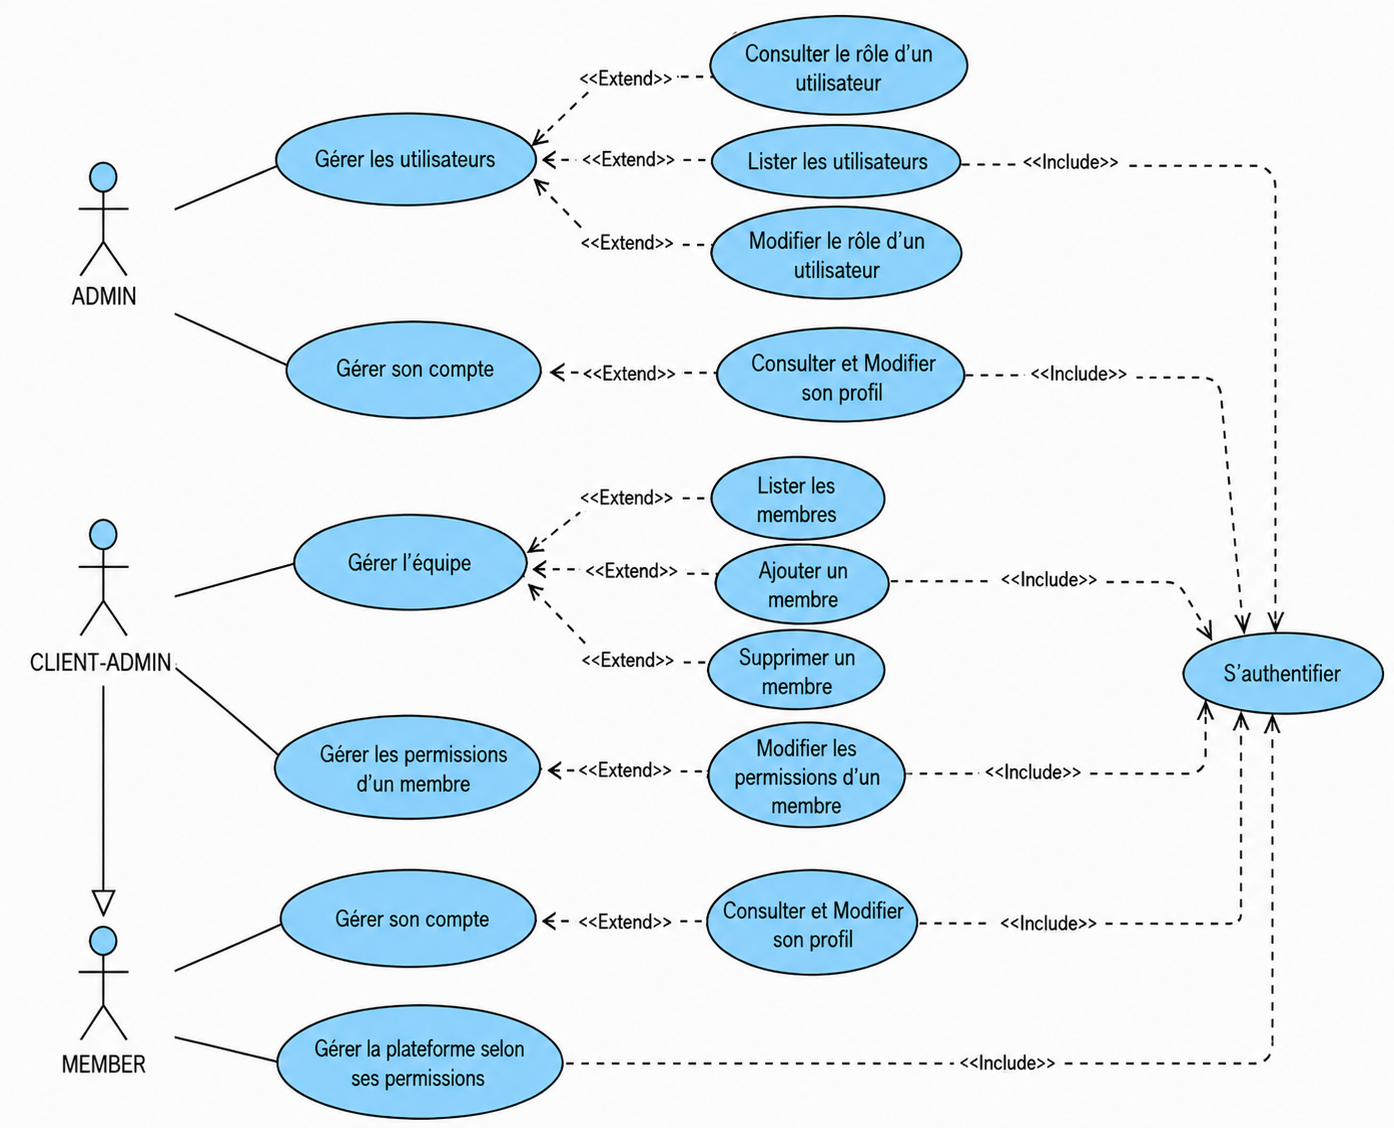
\includegraphics[width=0.85\textwidth]{image/uc-sprint3.png}
    \caption{Diagramme de cas d'utilisation du Sprint 3 — Gestion des utilisateurs et des accès}
    \label{fig:uc-sprint3}
\end{figure}

\subsection{Services Web}

\needspace{5cm}
\begin{longtable}{|p{6cm}|p{9.3cm}|}
\hline
Service Web & Description \\
\hline
\endfirsthead
\hline
Service Web & Description \\
\hline
\endhead
\hline
\endfoot
\endlastfoot
\texttt{POST /api/auth/register} & Créer un compte. \\ \hline
Connexion (Keycloak, OIDC) & Échange des identifiants contre un jeton, hors API du backend. \\ \hline
\texttt{GET /api/users/me} & Consulter son profil. \\ \hline
\texttt{PATCH /api/users/me} & Modifier son profil. \\ \hline
\texttt{GET /api/users} & Lister les utilisateurs (ADMIN). \\ \hline
\texttt{PATCH /api/users/\{id\}/role} & Modifier le rôle d'un utilisateur (ADMIN). \\ \hline
\texttt{GET /api/team/members} & Lister les membres de son équipe. \\ \hline
\texttt{POST /api/team/members} & Ajouter un membre. \\ \hline
\texttt{PUT /api/team/members/\{id\}/permissions} & Modifier les permissions d'un membre. \\ \hline
\texttt{DELETE /api/team/members/\{id\}} & Supprimer un membre. \\ \hline
\end{longtable}

\subsection{Conception}

Une fonctionnalité est détaillée : l'ajout d'un membre, la plus distinctive sur le plan métier de ce sprint, puisqu'elle ne suit pas un flux d'invitation classique.

\subsubsection{Cas d'utilisation : « Ajouter un membre »}

\subsubsection*{Description textuelle}

\needspace{8cm}
\renewcommand{\arraystretch}{1.5}
\begin{longtable}{|p{4cm}|p{11cm}|}
\hline
Nom & Ajouter un membre à son équipe \\
\hline
Acteur & CLIENT\_ADMIN \\
\hline
Pré-condition & Le CLIENT\_ADMIN est authentifié \\
\hline
Scénario nominal & 1. Le CLIENT\_ADMIN saisit le nom d'utilisateur, l'e-mail et le mot de passe du futur membre. \newline
2. Le backend crée le compte dans Keycloak, avec ce mot de passe marqué comme permanent. \newline
3. Le backend crée l'utilisateur local correspondant, rôle MEMBER, rattaché au compte du CLIENT\_ADMIN. \\
\hline
Post-condition & Le membre peut se connecter immédiatement avec les identifiants qui lui ont été transmis en dehors du système. \\
\hline
\caption{Description textuelle du cas d'utilisation « Ajouter un membre »}
\label{tab:uc-add-member}
\end{longtable}

Il ne s'agit pas d'un flux d'invitation par e-mail : le CLIENT\_ADMIN choisit lui-même les identifiants du membre, qu'il lui communique par un canal de son choix.

\subsubsection*{Diagramme de séquence}

\begin{figure}[H]
 \centering
    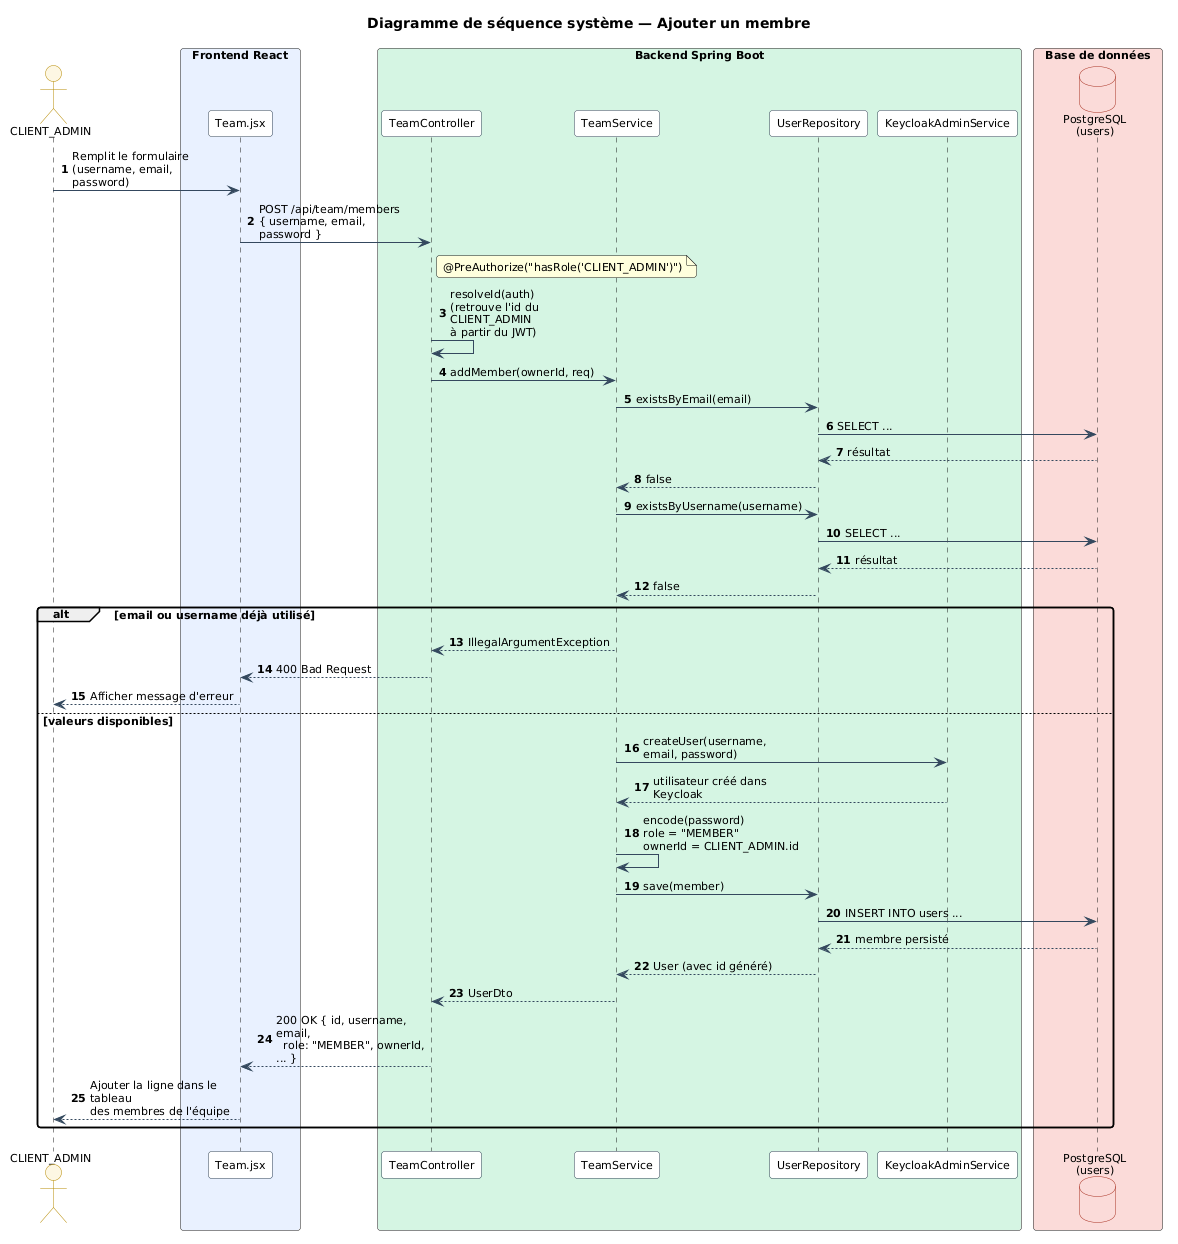
\includegraphics[width=0.7\textwidth]{image/seq-addmember.png}
    \caption{Diagramme de séquence — Ajouter un membre}
    \label{fig:seq-addmember}
\end{figure}

\subsection{Réalisation du Sprint 3}

Fonctionnalité : Créer un compte. Un visiteur peut créer un compte depuis le portail. Le rôle attribué par défaut est MEMBER, sans compte propriétaire : un tel compte ne peut effectuer aucune action tant qu'un ADMIN ne lui attribue pas un rôle actif.

Fonctionnalité : Se connecter. L'utilisateur se connecte avec son compte, quel que soit son rôle, depuis la même interface.

\begin{figure}[H]
 \centering
    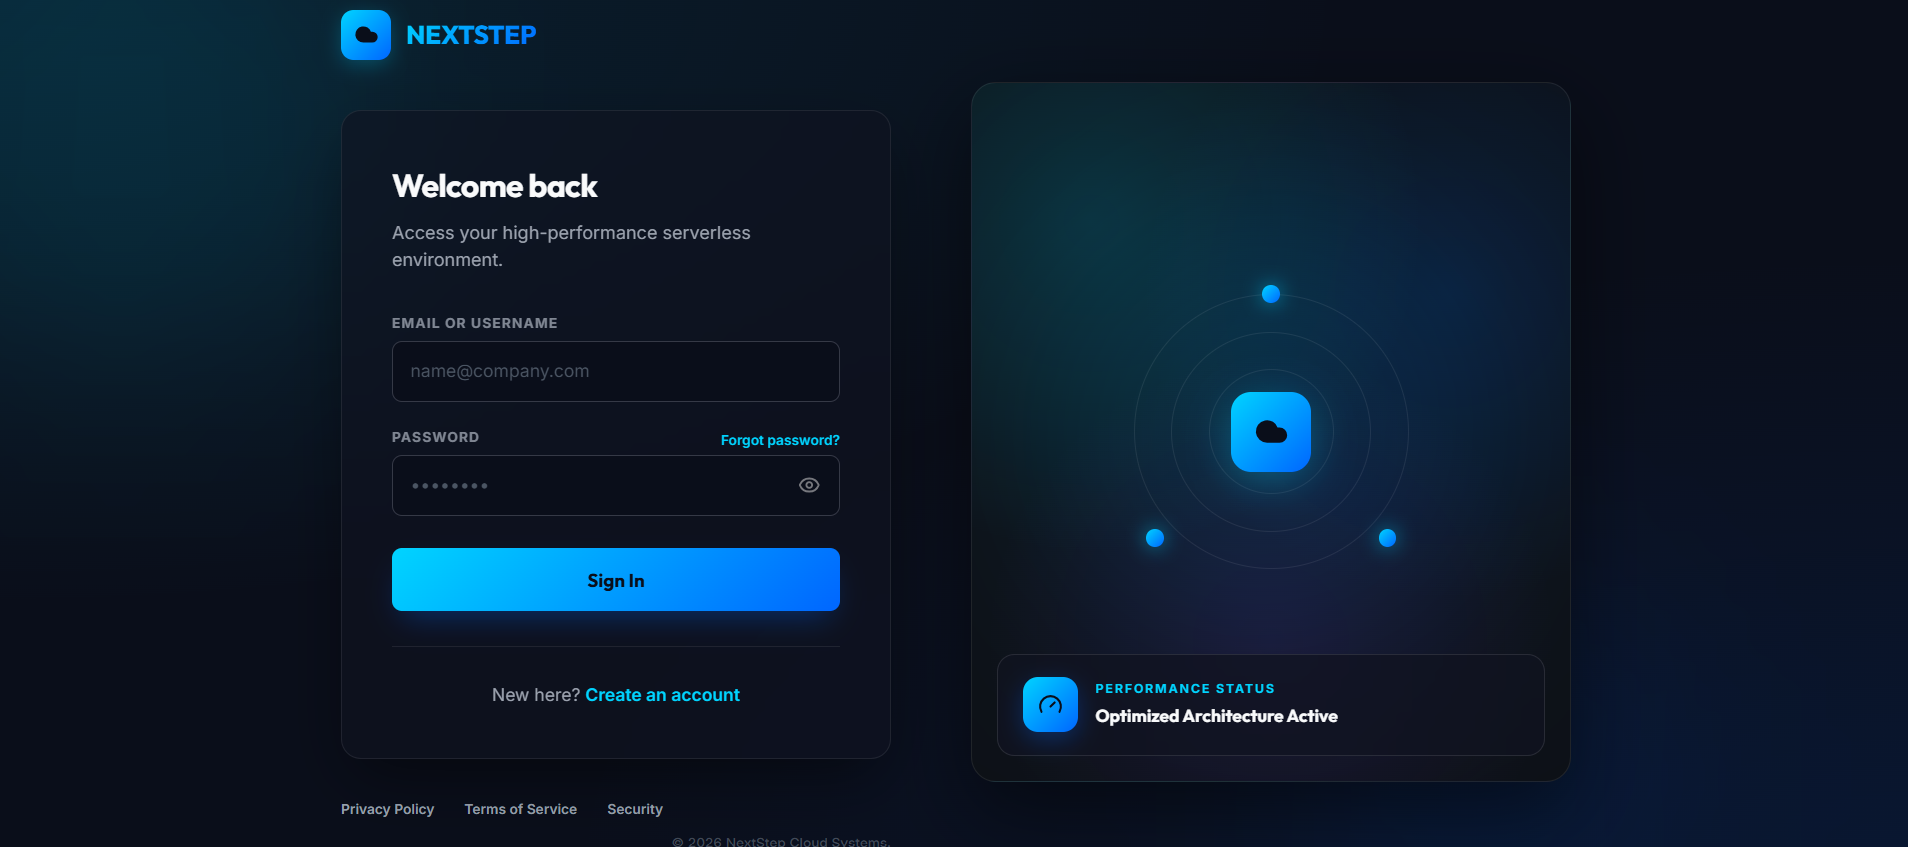
\includegraphics[width=\textwidth]{image/capture-login.png}
    \caption{Interface de connexion}
    \label{fig:capture-login}
\end{figure}

Fonctionnalité : Consulter et modifier son profil. Chaque utilisateur consulte et met à jour ses informations de profil depuis les paramètres de son compte.

\EmplacementFigure{13cm}{8cm}{Interface de gestion du profil}{fig:capture-profile}

Fonctionnalité : Gérer les utilisateurs (ADMIN). L'ADMIN consulte la liste des utilisateurs de la plateforme et modifie leur rôle depuis la console d'administration.

Fonctionnalité : Gérer son équipe (CLIENT\_ADMIN). Le CLIENT\_ADMIN consulte la liste des membres de son équipe, en ajoute, en supprime, et modifie leurs permissions individuellement.

\begin{figure}[H]
 \centering
    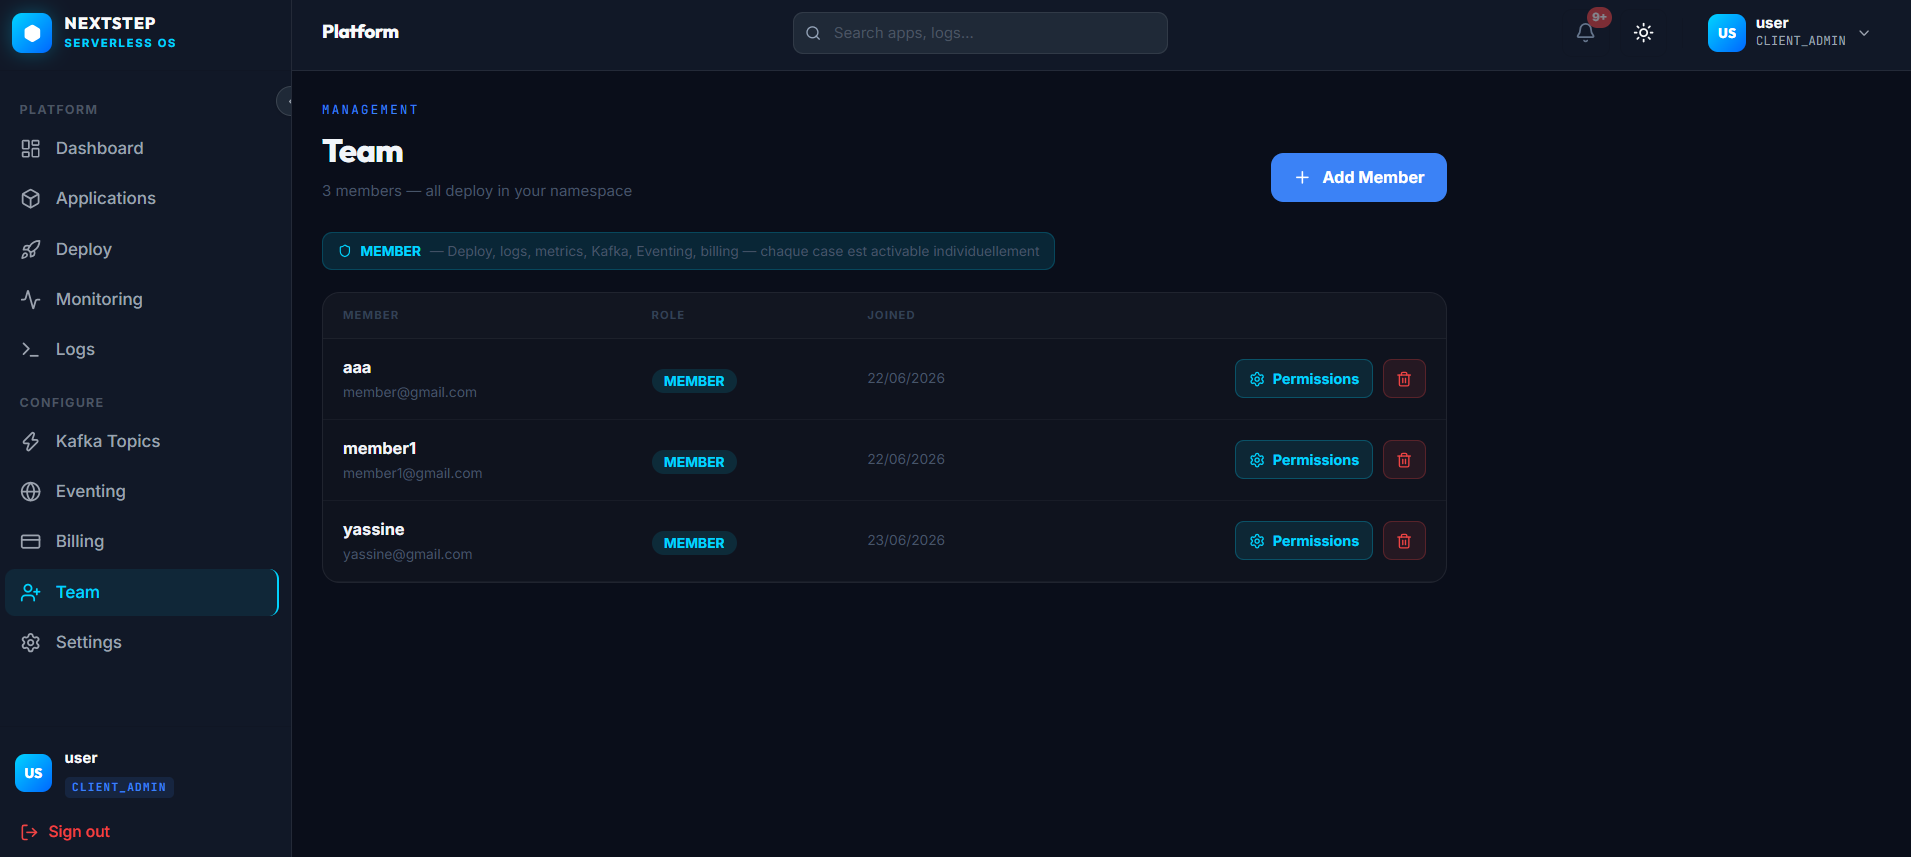
\includegraphics[width=\textwidth]{image/capture-team.png}
    \caption{Interface de gestion de l'équipe}
    \label{fig:capture-team}
\end{figure}

\subsection{Conclusion}

Ce sprint livre l'identité et le contrôle d'accès de la plateforme : connexion commune aux trois rôles, gestion des utilisateurs côté ADMIN, gestion d'équipe côté CLIENT\_ADMIN. Toutes les fonctionnalités développées dans les sprints suivants s'appuient sur ce socle de rôles et de permissions.

\clearpage
\section{Sprint 4 : Gestion des applications}

\subsection{Introduction}

Ce sprint livre le cycle de vie complet d'une application cliente : déploiement, consultation, mise à jour, suppression, historique des révisions et retour à une version antérieure, ainsi que les actions de suspension et de suppression forcée réservées à l'ADMIN. C'est la première fonctionnalité complète et accessible de bout en bout depuis le portail, appuyée sur les accès mis en place au Sprint 3 et sur Knative Serving (Release 0).

\subsection{Sprint Backlog}

Le tableau~\ref{tab:sb-sprint4} présente le backlog détaillé du Sprint 4, obtenu en décomposant chaque User Story retenue en tâches techniques.

\needspace{0.9\textheight}
{
\setlength{\LTleft}{-1.5cm}
\setlength{\LTright}{-1.5cm}
\setlength{\tabcolsep}{8pt}
\renewcommand{\arraystretch}{1.9}
\begin{longtable}{|p{6.6cm}|>{\raggedright\arraybackslash}p{8.1cm}|>{\centering\arraybackslash}p{2.3cm}|}
\hline
User Story & Tâches & Estimation \\
\hline
\endfirsthead
\hline
User Story & Tâches & Estimation \\
\hline
\endhead
\hline
\endfoot

\caption{Backlog du Sprint 4}
\label{tab:sb-sprint4}
\endlastfoot

\multirow{4}{6.6cm}{\centering En tant que CLIENT\_ADMIN ou MEMBER (avec permission DEPLOY\_APP), je veux déployer une application à partir d'une image Docker afin de la mettre en service.}
& Développer l'API de déploiement. & 1 \\* \cline{2-3}
& Développer le formulaire de déploiement du portail. & 1 \\* \cline{2-3}
& Intégrer la création de la ressource Knative correspondante. & 1 \\* \cline{2-3}
& Tester le déploiement d'une application. & 1 \\ \hline

\multirow{3}{6.6cm}{\centering En tant que CLIENT\_ADMIN ou MEMBER, je veux consulter mes applications et leur statut afin de suivre leur état.}
& Développer la liste des applications. & 1 \\* \cline{2-3}
& Développer la page de détail d'une application. & 1 \\* \cline{2-3}
& Synchroniser le statut en temps réel depuis Kubernetes. & 1 \\ \hline

\multirow{3}{6.6cm}{\centering En tant que CLIENT\_ADMIN ou MEMBER (avec permission DEPLOY\_APP/DELETE\_APP), je veux modifier, redéployer ou supprimer une application afin d'en gérer le cycle de vie.}
& Développer la mise à jour et le redéploiement. & 1 \\* \cline{2-3}
& Développer la suppression d'une application. & 1 \\* \cline{2-3}
& Tester la suppression et la mise à jour. & 1 \\ \hline

\multirow{3}{6.6cm}{\centering En tant que CLIENT\_ADMIN ou MEMBER (avec permission DEPLOY\_APP), je veux consulter l'historique des révisions et revenir à une version antérieure afin de corriger un déploiement défectueux.}
& Développer la liste des révisions. & 1 \\* \cline{2-3}
& Développer le retour à une révision antérieure. & 1 \\* \cline{2-3}
& Tester ce retour en arrière. & 1 \\ \hline

\multirow{3}{6.6cm}{\centering En tant qu'ADMIN, je veux suspendre, restaurer ou supprimer de force une application afin de gérer les abus ou incidents.}
& Développer la suspension et la restauration d'une application. & 1 \\* \cline{2-3}
& Développer la suppression forcée. & 1 \\* \cline{2-3}
& Tester ces actions administratives. & 1 \\ \hline

\end{longtable}
}

\subsection{Diagramme de cas d'utilisation du Sprint 4}

Le diagramme réunit CLIENT\_ADMIN et MEMBER (généralisés sous « Utilisateur du compte », les actions de MEMBER étant conditionnées par les permissions \texttt{DEPLOY\_APP}/\texttt{DELETE\_APP}) et ADMIN, avec l'ensemble des fonctionnalités du sprint.

\begin{figure}[H]
 \centering
    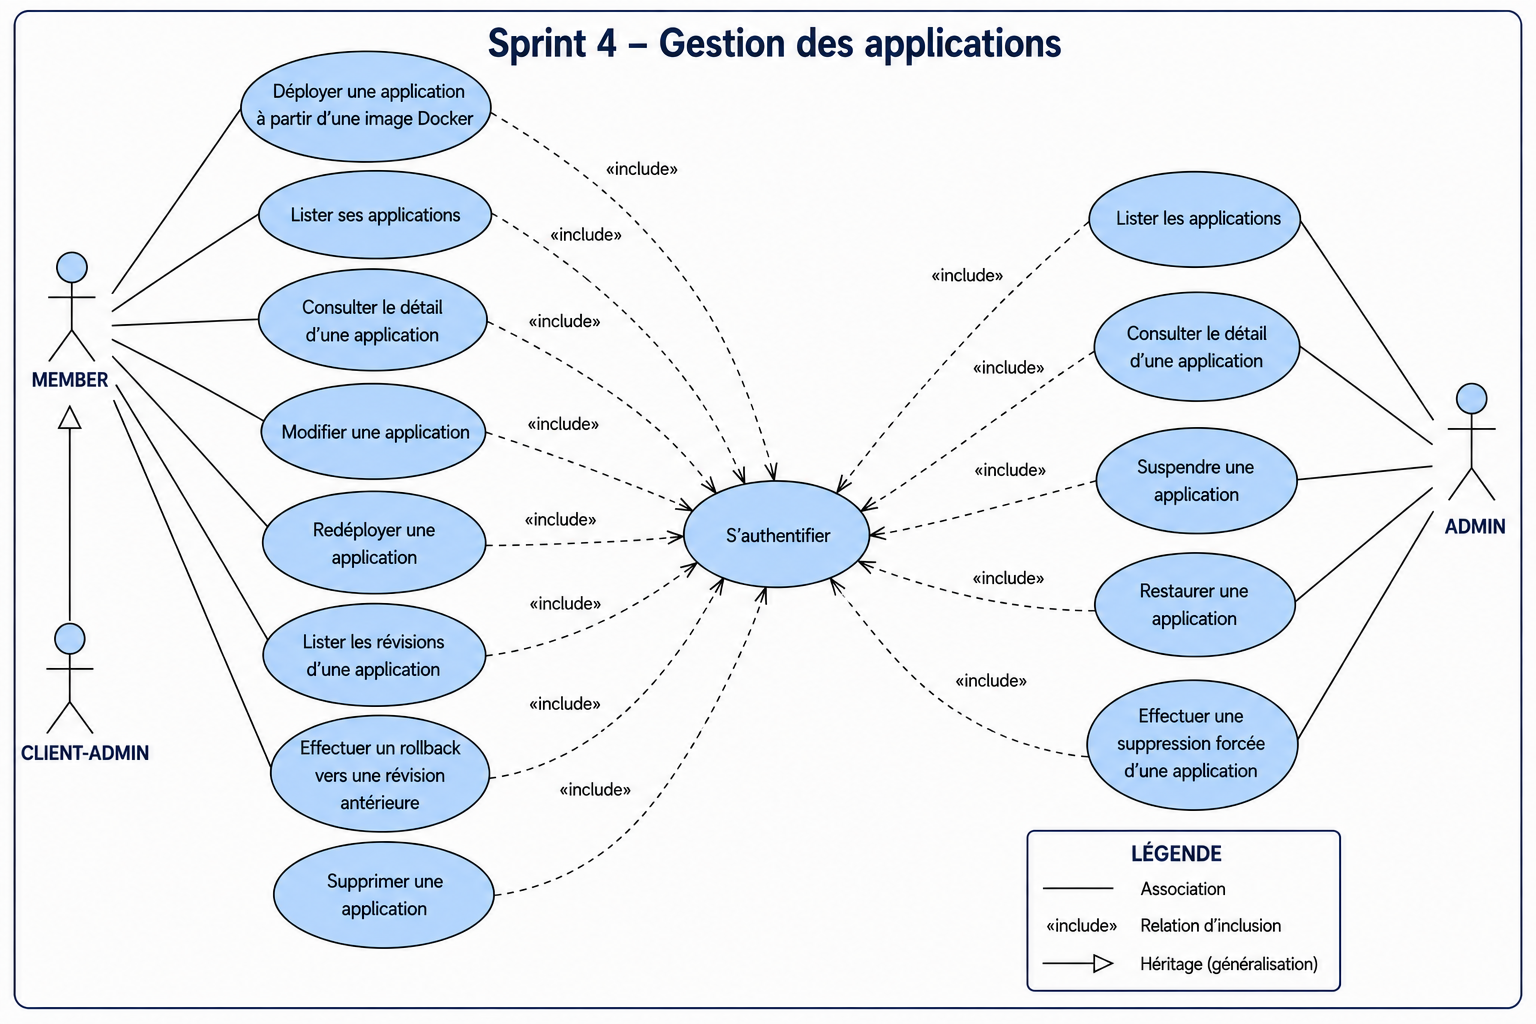
\includegraphics[width=0.95\textwidth]{image/uc-sprint4.png}
    \caption{Diagramme de cas d'utilisation du Sprint 4 — Gestion des applications}
    \label{fig:uc-sprint4}
\end{figure}

\subsection{Services Web}

\needspace{5cm}
\begin{longtable}{|p{6cm}|p{9.3cm}|}
\hline
Service Web & Description \\
\hline
\endfirsthead
\hline
Service Web & Description \\
\hline
\endhead
\hline
\endfoot
\endlastfoot
\texttt{POST /api/apps} & Déployer une application. \\ \hline
\texttt{GET /api/apps} & Lister ses applications. \\ \hline
\texttt{GET /api/apps/\{id\}} & Détail d'une application. \\ \hline
\texttt{POST /api/apps/\{id\}/deploy} & Redéployer une application existante. \\ \hline
\texttt{PUT /api/apps/\{id\}} & Modifier une application. \\ \hline
\texttt{DELETE /api/apps/\{id\}} & Supprimer une application. \\ \hline
\texttt{GET /api/apps/\{id\}/revisions} & Lister les révisions. \\ \hline
\texttt{POST /api/apps/\{id\}/rollback/\{revisionName\}} & Revenir à une révision antérieure. \\ \hline
\texttt{GET /api/admin/apps} & Lister toutes les applications, tous locataires confondus (ADMIN). \\ \hline
\texttt{DELETE /api/admin/apps/\{id\}} & Suppression forcée (ADMIN). \\ \hline
\texttt{POST /api/admin/apps/\{id\}/suspend} & Suspendre une application (ADMIN). \\ \hline
\texttt{POST /api/admin/apps/\{id\}/restore} & Restaurer une application suspendue (ADMIN). \\ \hline
\end{longtable}

\subsection{Conception}

Deux fonctionnalités sont détaillées : le déploiement, cœur fonctionnel du sprint et de la plateforme ; le retour à une révision antérieure, scénario opérationnel distinctif.

\subsubsection{Cas d'utilisation : « Déployer une application »}

\subsubsection*{Description textuelle}

\renewcommand{\arraystretch}{1.5}
\begin{longtable}{|p{4cm}|p{11cm}|}
\hline
Nom & Déployer une application \\
\hline
Acteur & CLIENT\_ADMIN, MEMBER (avec permission de déploiement) \\
\hline
Pré-condition & L'utilisateur est authentifié et dispose de la permission de déploiement \\
\hline
Scénario nominal & 1. L'utilisateur renseigne le formulaire de déploiement (nom, image, port, ressources, bornes de mise à l'échelle). 2. L'application est créée avec un statut de déploiement en cours. 3. Le backend répond immédiatement, puis déclenche de manière asynchrone la création de la ressource Knative correspondante. 4. Le statut de l'application est mis à jour en temps réel à mesure que Knative provisionne le service. \\
\hline
Post-condition & L'application est déployée et accessible, ou son statut reflète l'échec du déploiement. \\
\hline
\caption{Description textuelle du cas d'utilisation « Déployer une application »}
\label{tab:uc-deploy}
\end{longtable}

\subsubsection*{Diagramme de séquence}

\begin{figure}[H]
 \centering
    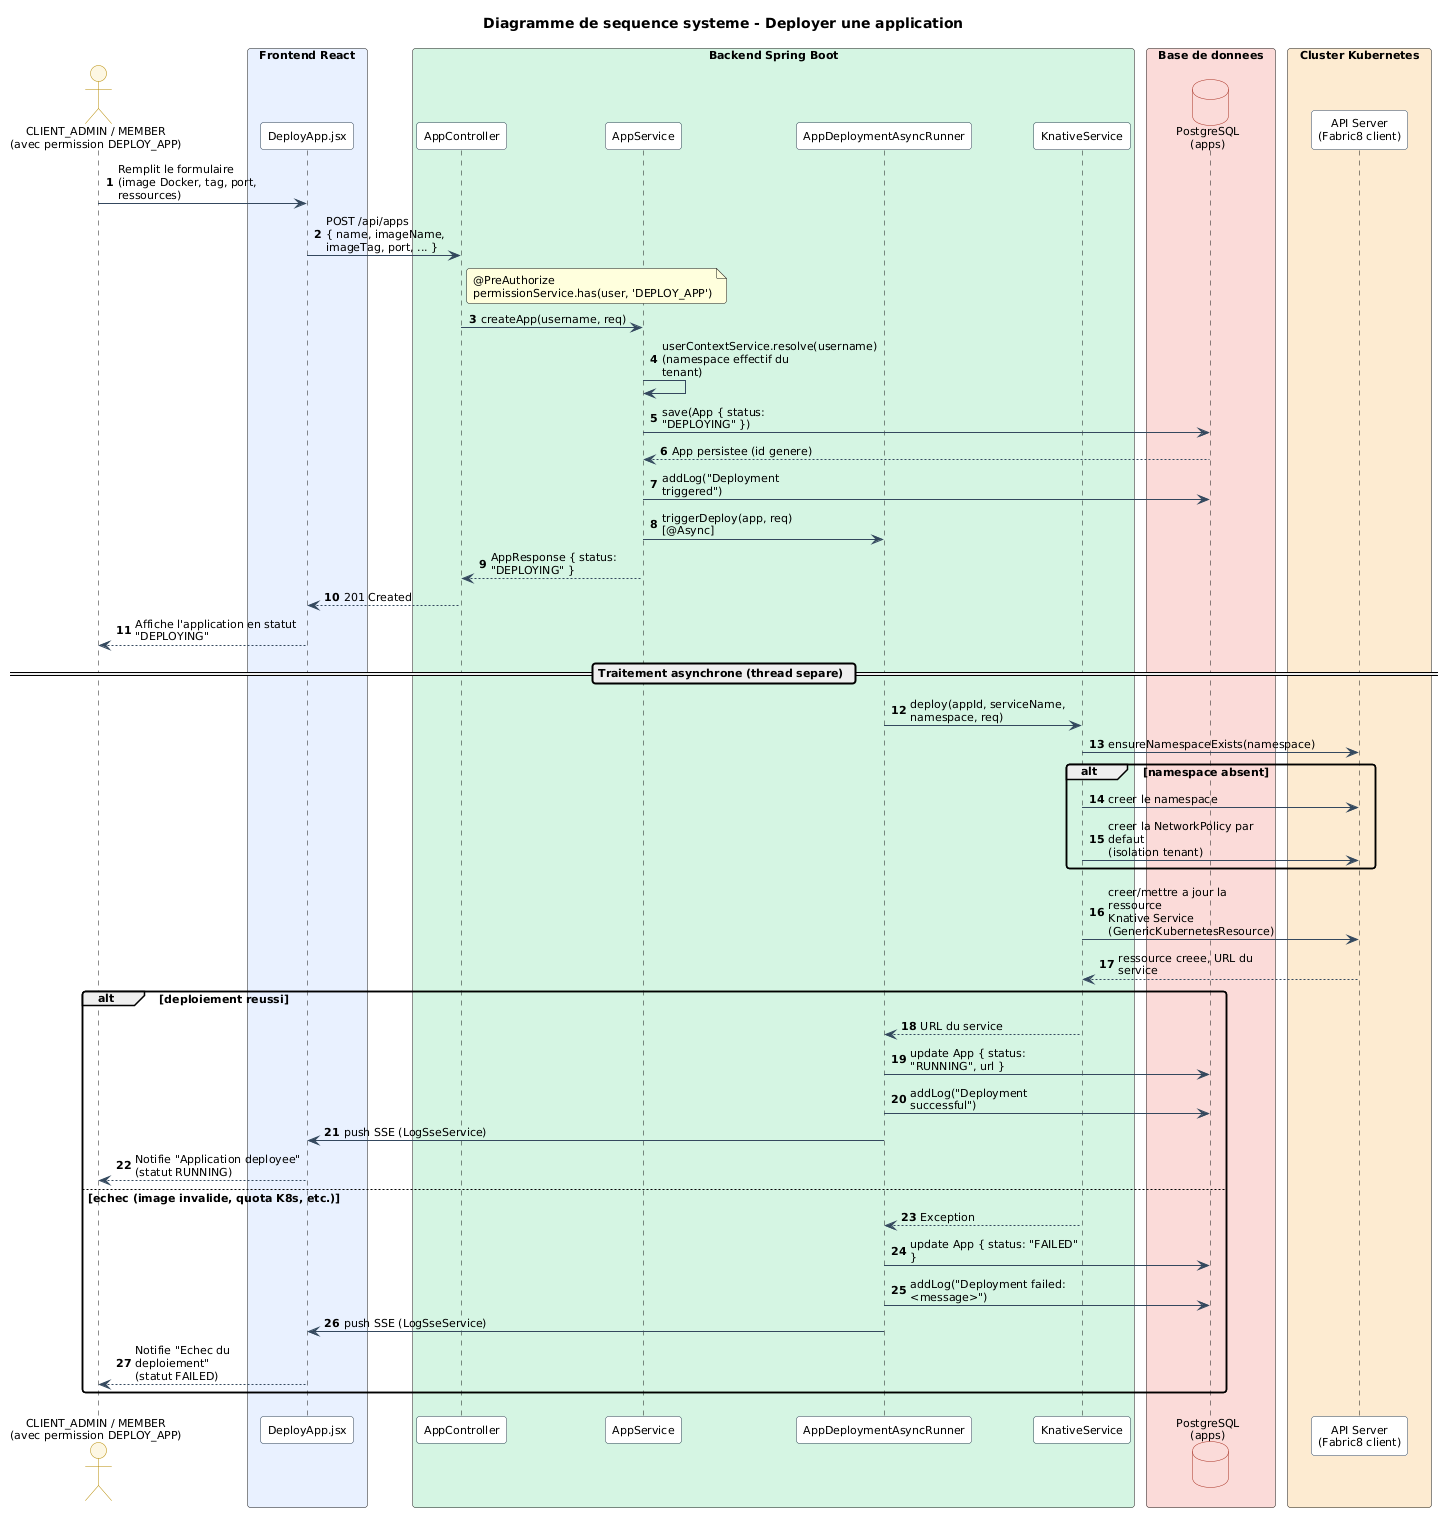
\includegraphics[width=\textwidth,height=0.85\textheight,keepaspectratio]{image/seq-deploy.png}
    \caption{Diagramme de séquence — Déployer une application}
    \label{fig:seq-deploy}
\end{figure}

\subsubsection{Cas d'utilisation : « Revenir à une révision antérieure »}

\subsubsection*{Description textuelle}

\renewcommand{\arraystretch}{1.5}
\begin{longtable}{|p{4cm}|p{11cm}|}
\hline
Nom & Revenir à une révision antérieure \\
\hline
Acteur & CLIENT\_ADMIN, MEMBER (avec permission de déploiement) \\
\hline
Pré-condition & L'application dispose d'au moins deux révisions \\
\hline
Scénario nominal & 1. L'utilisateur consulte l'historique des révisions de son application. 2. Il sélectionne une révision antérieure. 3. Le backend fait pointer le trafic Knative vers cette révision. \\
\hline
Post-condition & L'application sert à nouveau le comportement de la révision sélectionnée. \\
\hline
\caption{Description textuelle du cas d'utilisation « Revenir à une révision antérieure »}
\label{tab:uc-rollback}
\end{longtable}

\subsubsection*{Diagramme de séquence}

\begin{figure}[H]
 \centering
    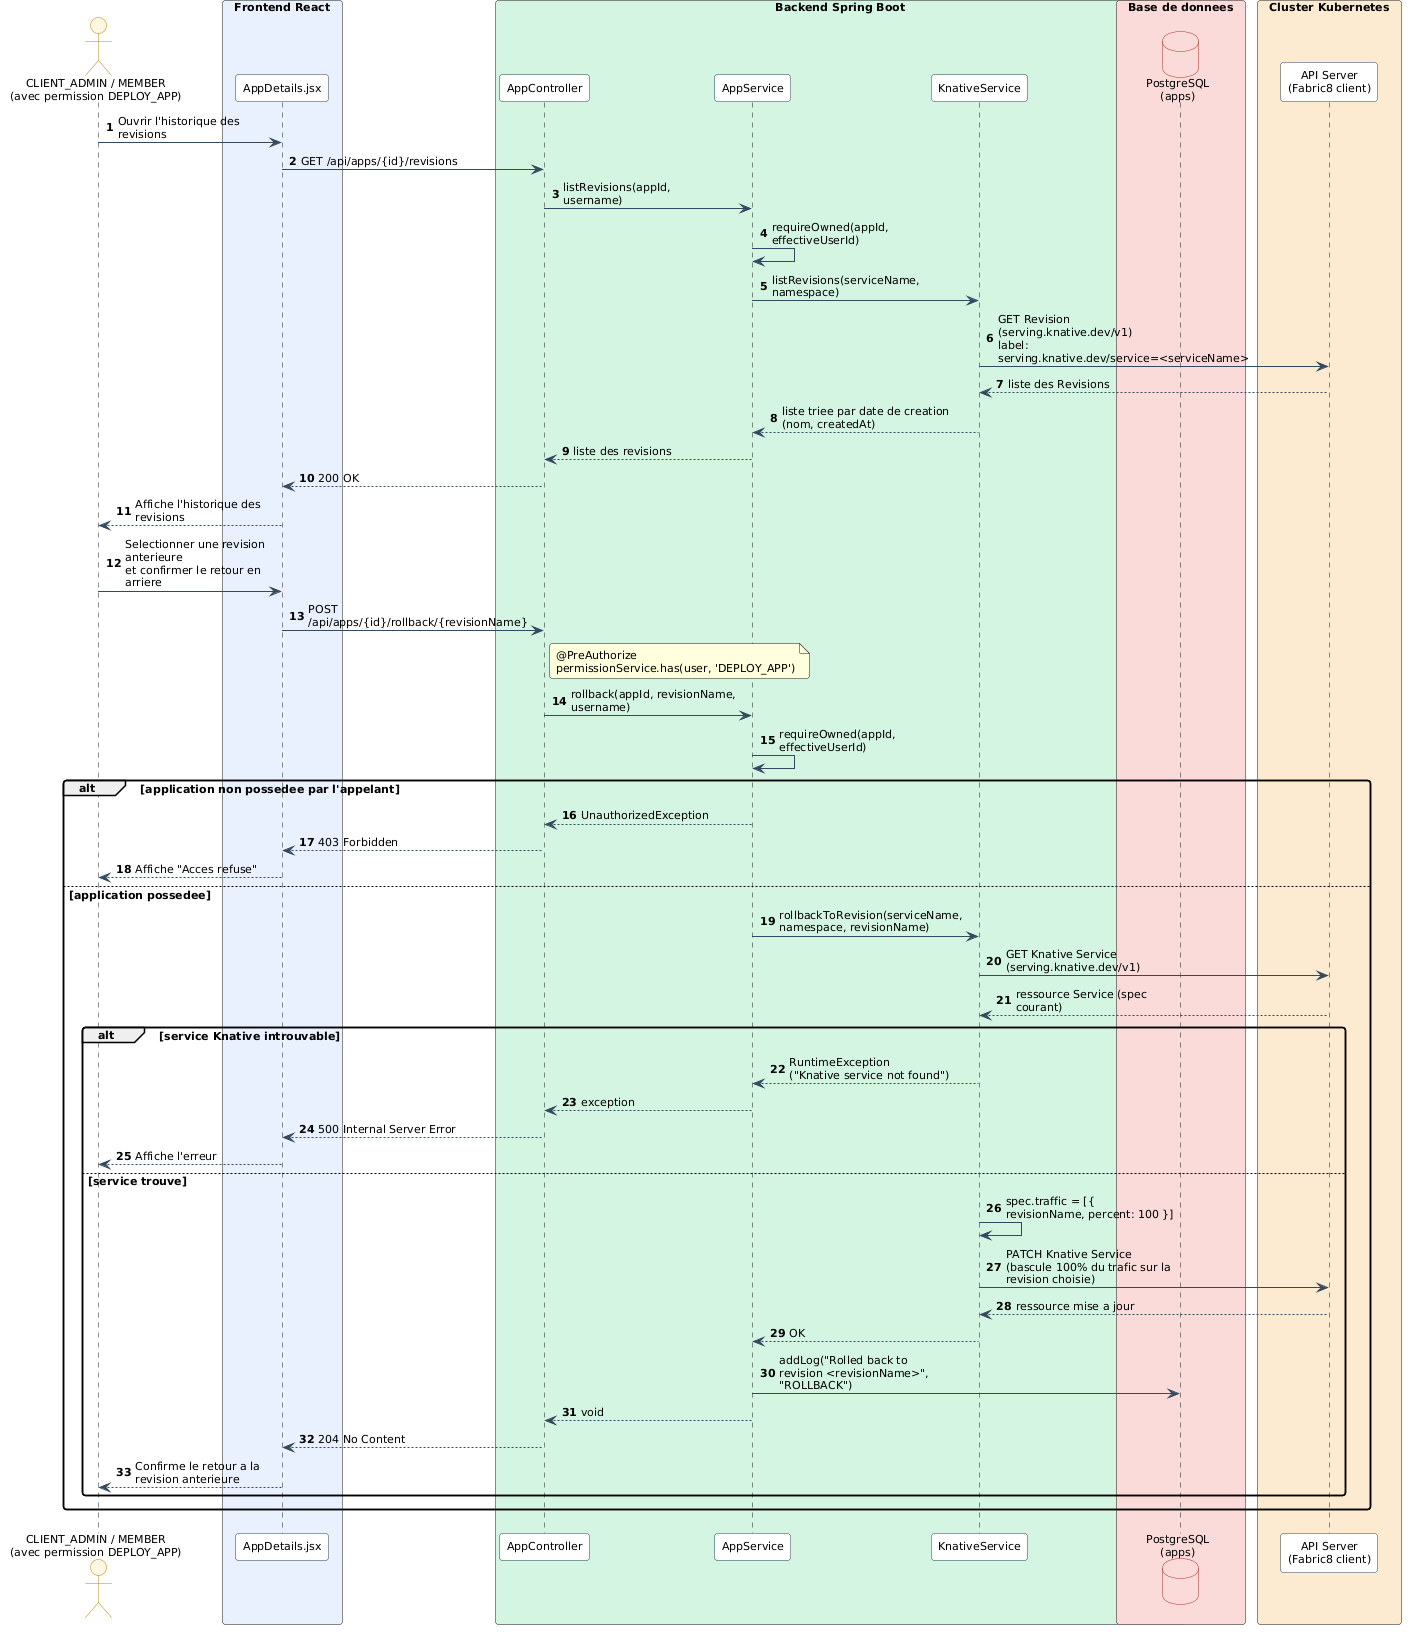
\includegraphics[width=\textwidth,height=0.85\textheight,keepaspectratio]{image/seq-rollback.png}
    \caption{Diagramme de séquence — Revenir à une révision antérieure}
    \label{fig:seq-rollback}
\end{figure}

\subsection{Réalisation du Sprint 4}

Fonctionnalité : Déployer une application. Le formulaire de déploiement du portail permet de créer une application à partir d'une image Docker.

\begin{figure}[H]
 \centering
    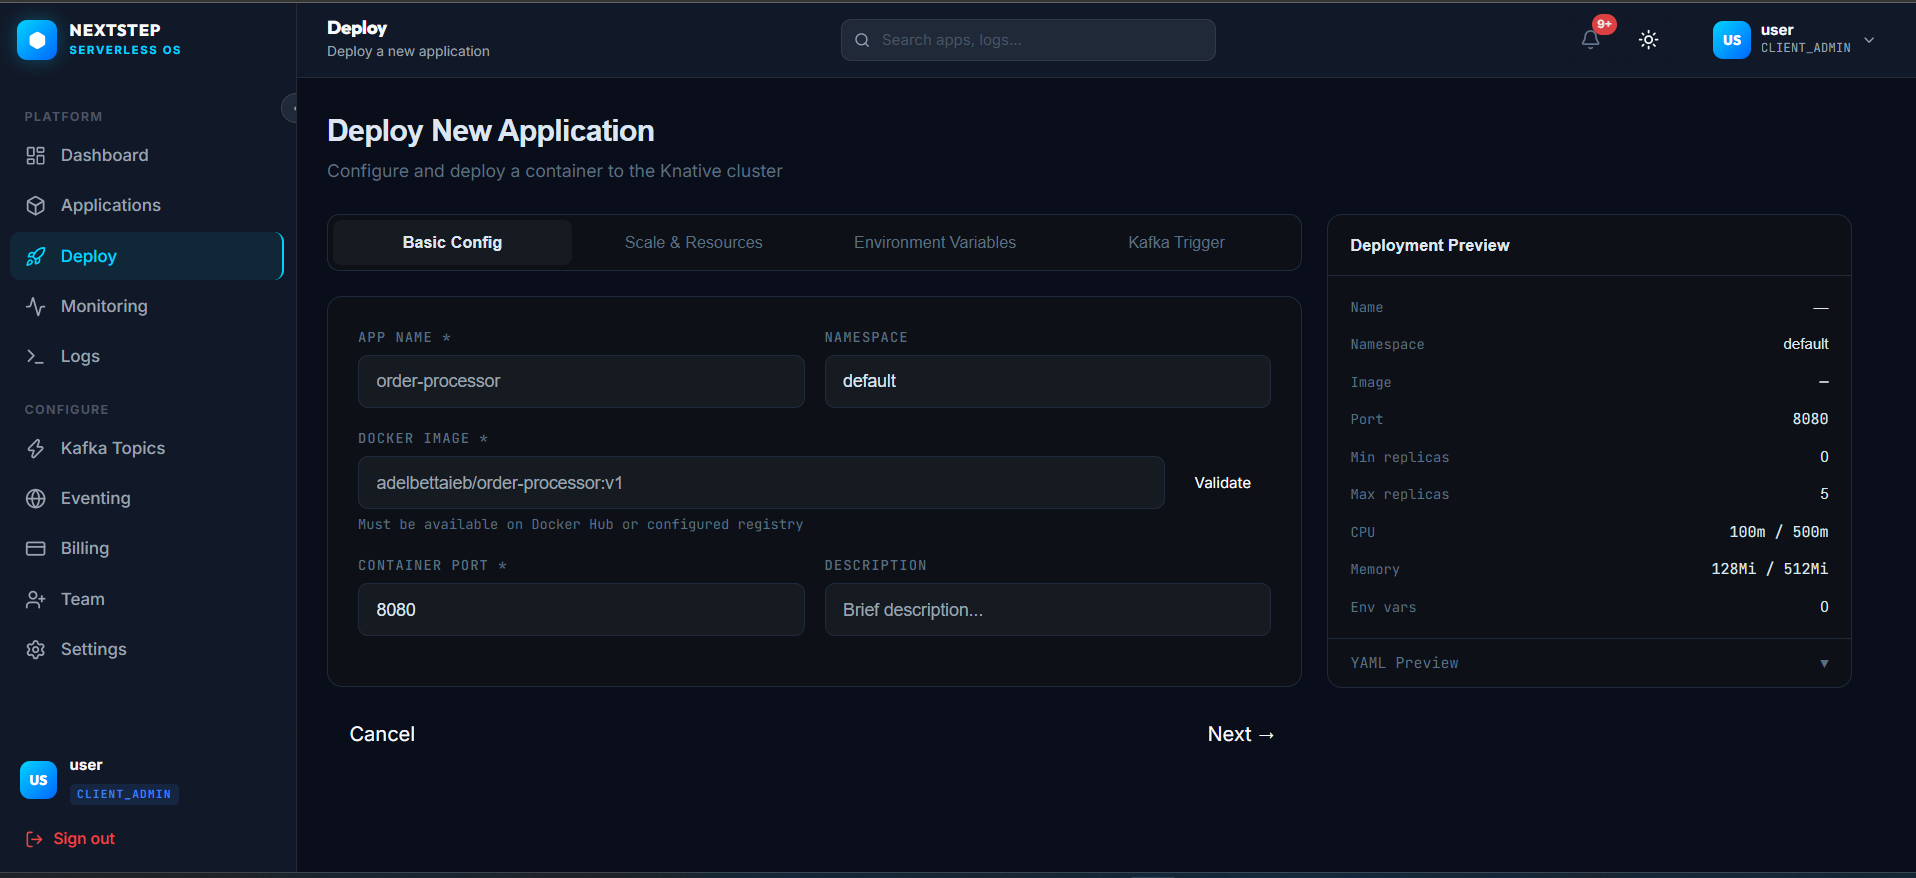
\includegraphics[width=\textwidth]{image/capture-deploy.png}
    \caption{Formulaire de déploiement d'une application}
    \label{fig:capture-deploy}
\end{figure}

Fonctionnalité : Consulter ses applications et leur statut. Le tableau de bord liste les applications du compte avec leur statut, synchronisé en temps réel depuis le cluster.

\begin{figure}[H]
 \centering
    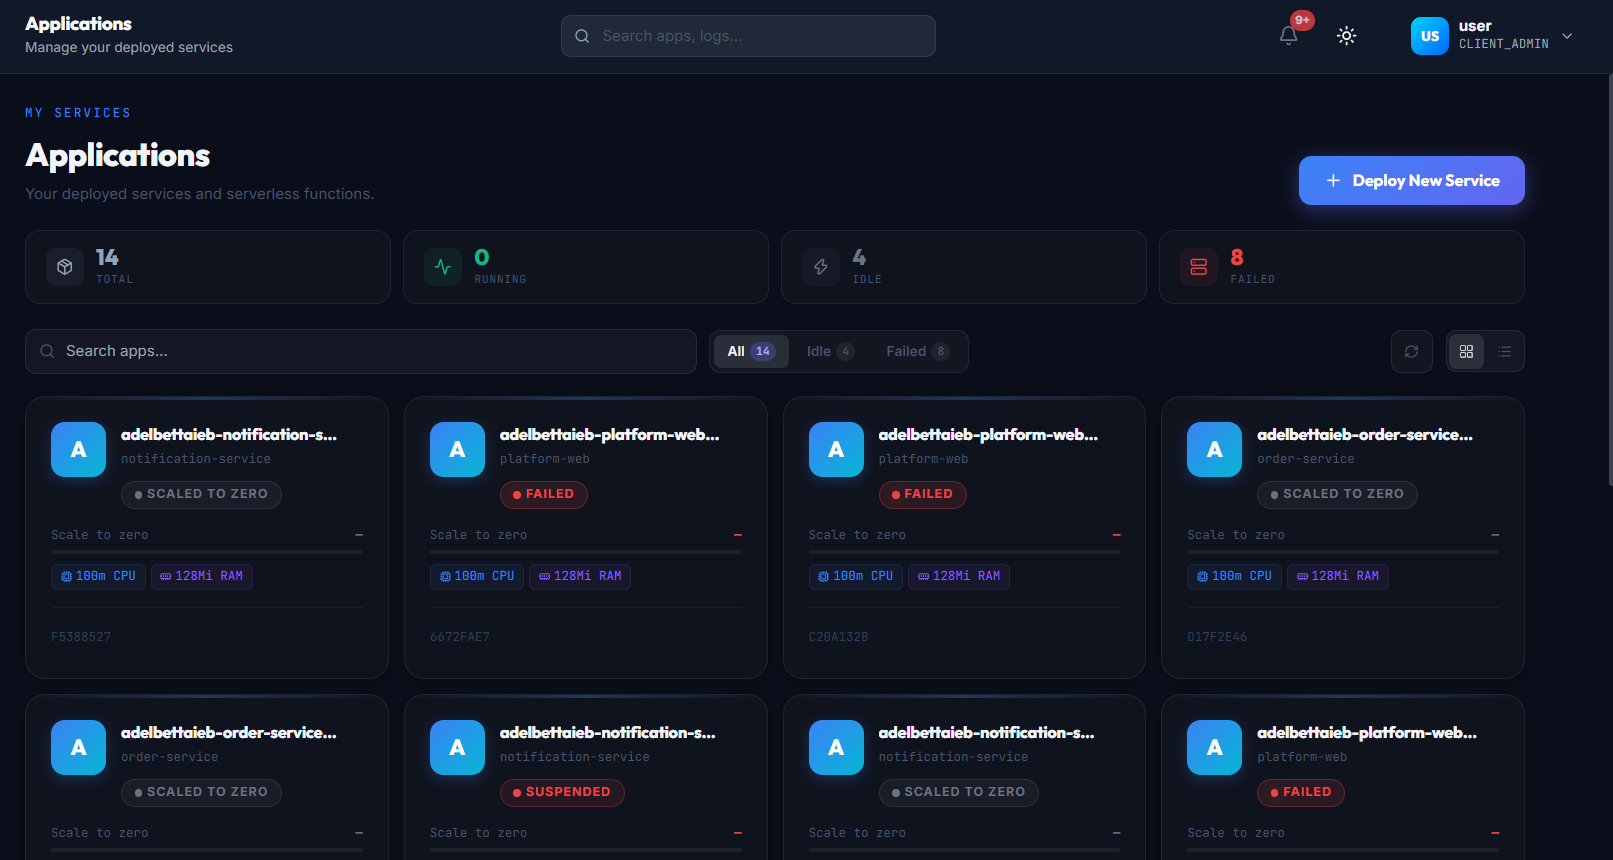
\includegraphics[width=\textwidth]{image/capture-appslist.png}
    \caption{Liste des applications et de leur statut}
    \label{fig:capture-appslist}
\end{figure}

Fonctionnalité : Modifier, redéployer ou supprimer une application. La page de détail d'une application permet de la modifier, de la redéployer ou de la supprimer.

Fonctionnalité : Consulter l'historique des révisions et revenir en arrière. L'historique des révisions et le retour à une version antérieure sont accessibles depuis la page de détail.

Fonctionnalité : Suspendre ou supprimer de force une application (ADMIN). L'ADMIN dispose, depuis la console d'administration, d'actions de suspension et de suppression forcée sur n'importe quelle application.

\EmplacementFigure{13cm}{8cm}{Actions administratives sur une application}{fig:capture-adminapps}

Au-delà du scénario nominal, le déploiement peut, si le formulaire renseigne un sujet Kafka, câbler automatiquement l'application créée à ce sujet, sans étape manuelle supplémentaire : ce chemin optionnel est décrit avec la gestion de la messagerie événementielle (Sprint 5), dont il anticipe la fonctionnalité de configuration d'un déclencheur.

\subsection{Conclusion}

Ce sprint livre le cycle de vie complet de gestion d'une application, accessible depuis le portail, avec un déploiement asynchrone et un suivi de statut en temps réel. La gestion des applications sert de socle à la messagerie événementielle et à l'observabilité applicative, objets des deux sprints suivants.

\clearpage
\section{Sprint 5 : Gestion de la messagerie événementielle}

\subsection{Introduction}

Ce sprint livre, comme un seul domaine fonctionnel, la gestion des sujets Kafka et la configuration des déclencheurs qui relient un sujet à une application : la publication d'un message sur un sujet réveille alors automatiquement l'application concernée. Ces deux briques, Kafka (Strimzi) et Knative Eventing, ne prennent leur sens qu'ensemble ; les traiter comme un seul sprint évite de les documenter à deux endroits distincts.

\subsection{Sprint Backlog}

Le tableau~\ref{tab:sb-sprint5} présente le backlog détaillé du Sprint 5, obtenu en décomposant chaque User Story retenue en tâches techniques.

\needspace{0.9\textheight}
{
\setlength{\LTleft}{-1.5cm}
\setlength{\LTright}{-1.5cm}
\setlength{\tabcolsep}{8pt}
\renewcommand{\arraystretch}{1.9}
\begin{longtable}{|p{6.6cm}|>{\raggedright\arraybackslash}p{8.1cm}|>{\centering\arraybackslash}p{2.3cm}|}
\hline
User Story & Tâches & Estimation \\
\hline
\endfirsthead
\hline
User Story & Tâches & Estimation \\
\hline
\endhead
\hline
\endfoot

\caption{Backlog du Sprint 5}
\label{tab:sb-sprint5}
\endlastfoot

\multirow{4}{6.6cm}{\centering En tant que CLIENT\_ADMIN ou MEMBER (avec permission MANAGE\_KAFKA), je veux créer et gérer des sujets Kafka afin d'y publier des événements.}
& Développer la création d'un sujet Kafka. & 1 \\* \cline{2-3}
& Développer la liste et le détail d'un sujet. & 1 \\* \cline{2-3}
& Développer la suppression d'un sujet. & 1 \\* \cline{2-3}
& Développer la page de gestion des sujets Kafka. & 1 \\ \hline

\multirow{5}{6.6cm}{\centering En tant que CLIENT\_ADMIN ou MEMBER (avec permission MANAGE\_EVENTING), je veux relier un sujet Kafka à une application afin qu'elle soit réveillée automatiquement à la réception d'un message.}
& Développer la création d'une KafkaSource. & 1 \\* \cline{2-3}
& Développer la création d'un Trigger. & 1 \\* \cline{2-3}
& Développer la suppression d'un Trigger. & 1 \\* \cline{2-3}
& Développer la page de configuration des déclencheurs. & 1 \\* \cline{2-3}
& Tester le déclenchement d'une application. & 1 \\ \hline

\multirow{2}{6.6cm}{\centering En tant que CLIENT\_ADMIN ou MEMBER, je veux publier un événement sur un sujet afin de déclencher un traitement.}
& Développer l'API de publication d'un événement. & 1 \\* \cline{2-3}
& Tester la publication d'un événement. & 1 \\ \hline

\multirow{3}{6.6cm}{\centering En tant qu'ADMIN, je veux consulter l'ensemble des sujets, sources et déclencheurs de tous les clients, et supprimer un sujet de force, afin de gérer les abus.}
& Développer la vue globale des sujets, sources et déclencheurs. & 1 \\* \cline{2-3}
& Développer la suppression forcée d'un sujet. & 1 \\* \cline{2-3}
& Tester ces actions. & 1 \\ \hline

\end{longtable}
}

\subsection{Diagramme de cas d'utilisation du Sprint 5}

Le diagramme réunit CLIENT\_ADMIN et MEMBER (sous permission \texttt{MANAGE\_KAFKA}/\texttt{MANAGE\_EVENTING}), ainsi qu'ADMIN, avec l'ensemble des fonctionnalités du sprint.

\begin{figure}[H]
 \centering
    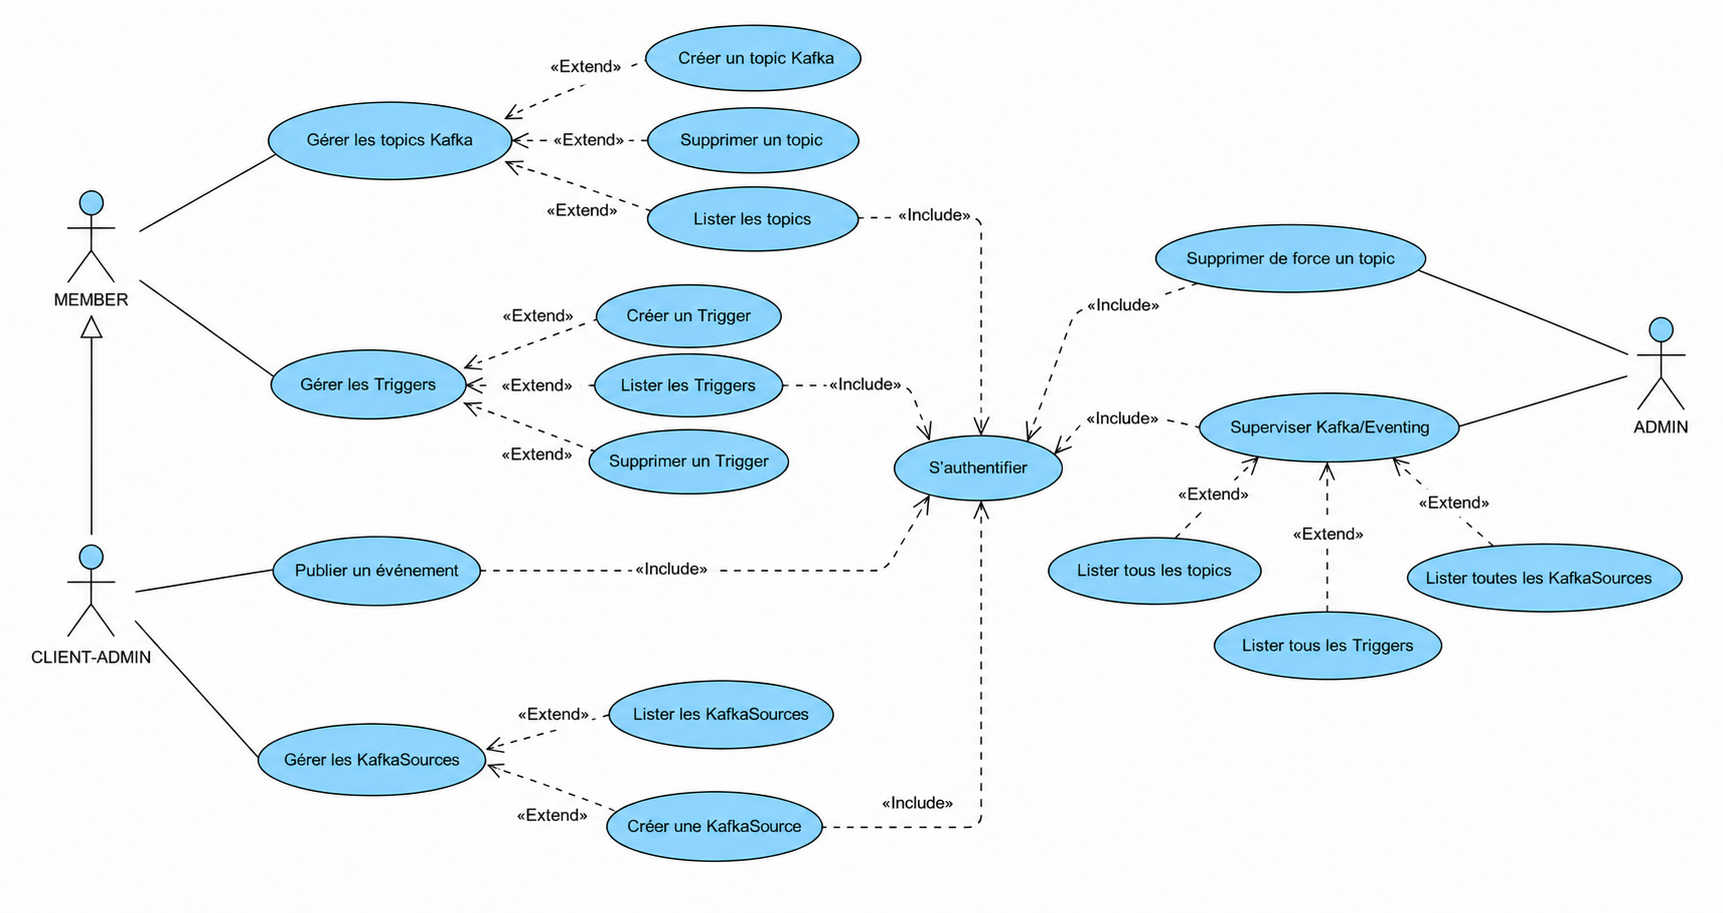
\includegraphics[width=\textwidth]{image/Sprint5usescase.png}
    \caption{Diagramme de cas d'utilisation du Sprint 5 — Gestion de la messagerie événementielle}
    \label{fig:uc-sprint5}
\end{figure}


\subsection{Services Web}

\needspace{5cm}
\begin{longtable}{|p{6cm}|p{9.3cm}|}
\hline
Service Web & Description \\
\hline
\endfirsthead
\hline
Service Web & Description \\
\hline
\endhead
\hline
\endfoot
\endlastfoot
\texttt{POST /api/kafka/topics} & Créer un sujet Kafka. \\ \hline
\texttt{GET /api/kafka/topics} & Lister ses sujets. \\ \hline
\texttt{GET /api/kafka/topics/\{id\}} & Détail d'un sujet. \\ \hline
\texttt{DELETE /api/kafka/topics/\{id\}} & Supprimer un sujet. \\ \hline
\texttt{POST /api/eventing/sources} & Créer une KafkaSource. \\ \hline
\texttt{GET /api/eventing/sources} & Lister ses KafkaSource. \\ \hline
\texttt{POST /api/eventing/triggers} & Créer un déclencheur (Trigger). \\ \hline
\texttt{GET /api/eventing/triggers} & Lister ses déclencheurs. \\ \hline
\texttt{DELETE /api/eventing/triggers/\{id\}} & Supprimer un déclencheur. \\ \hline
\texttt{POST /api/events} & Publier un événement (CloudEvent). \\ \hline
\texttt{GET /api/admin/kafka/topics} & Lister tous les sujets, tous locataires confondus (ADMIN). \\ \hline
\texttt{DELETE /api/admin/kafka/topics/\{id\}} & Suppression forcée d'un sujet (ADMIN). \\ \hline
\texttt{GET /api/admin/eventing/sources}, \texttt{/triggers} & Vue globale des sources et déclencheurs (ADMIN). \\ \hline
\end{longtable}

\subsection{Conception}

Une fonctionnalité est détaillée : la configuration d'un déclencheur, la plus riche techniquement puisqu'elle relie deux briques indépendantes du socle (Kafka et Knative).

\subsubsection{Cas d'utilisation : « Configurer un déclencheur d'événement »}

\subsubsection*{Description textuelle}

\renewcommand{\arraystretch}{1.5}
\begin{longtable}{|p{4cm}|p{11cm}|}
\hline
Nom & Configurer un déclencheur d'événement \\
\hline
Acteur & CLIENT\_ADMIN, MEMBER (avec permission de gestion de l'Eventing) \\
\hline
Pré-condition & L'application cible est déployée ; le sujet Kafka source existe \\
\hline
Scénario nominal & 1. L'utilisateur sélectionne un sujet Kafka et une application cible. 2. Le backend crée la ressource KafkaSource rattachée au sujet. 3. Le backend crée la ressource Trigger associée, filtrant sur le type d'événement et pointant vers l'URL du service Knative de l'application. 4. La configuration est persistée et son état est renvoyé à l'utilisateur. \\
\hline
Post-condition & Toute publication ultérieure sur le sujet Kafka déclenche, le cas échéant, le réveil et l'invocation de l'application. \\
\hline
\caption{Description textuelle du cas d'utilisation « Configurer un déclencheur d'événement »}
\label{tab:uc-eventing}
\end{longtable}

Ce processus, du message Kafka au réveil et au traitement par l'application, est illustré à la figure~\ref{fig:seq-eventing}.

\begin{figure}[H]
\begin{adjustwidth}{-1.3cm}{-1.3cm}
\centering
\begin{tikzpicture}[
  x=1cm, y=1cm,
  every node/.style={font=\normalsize},
  act/.style={draw=black!60, line width=1pt, rounded corners, minimum width=5.4cm,
              minimum height=1.3cm, align=center, fill=black!5},
  don/.style={draw=figBleu, line width=1pt, rounded corners, minimum width=5.4cm,
              minimum height=1.3cm, align=center, fill=figBleuFond},
  eta/.style={draw=figVert, line width=1pt, rounded corners, minimum width=5.4cm,
              minimum height=1.3cm, align=center, fill=figVertFond},
  ctl/.style={draw=figOrange, line width=1pt, dashed, rounded corners, minimum width=5.0cm,
              minimum height=1.3cm, align=center, fill=figOrangeFond},
  num/.style={circle, draw, line width=0.8pt, fill=white, inner sep=1.5pt, font=\small\bfseries},
  lbl/.style={font=\footnotesize},
  fl/.style={->, line width=1pt, figBleu},
  fv/.style={->, line width=1pt, figVert},
  fc/.style={->, line width=1pt, dashed, figOrange}
]

\node[act] (prod) at (0,0)     {Producteur\\[1pt]\small publie un message};
\node[don] (topic) at (0,-2.3)  {Sujet Kafka (cluster Strimzi)};
\node[don] (src)  at (0,-4.6)  {KafkaSource\\[1pt]\small consomme et encapsule en CloudEvent};
\node[don] (brk)  at (0,-6.9)  {Broker Knative Eventing};
\node[don] (trg)  at (0,-9.2)  {Trigger\\[1pt]\small filtre et route l'événement};
\node[eta] (pod)  at (0,-13.4) {Pod applicatif\\[1pt]\small traite l'événement, répond HTTP 200};
\node[eta] (fin)  at (0,-16.1) {Retour au repos\\[1pt]\small 0 instance après inactivité};

\node[ctl] (act)  at (9.4,-9.2)  {Activator\\[1pt]\small intercepte si 0 instance};
\node[ctl] (kpa)  at (9.4,-11.3) {Autoscaler (KPA)};
\node[ctl] (rev)  at (9.4,-13.4) {Revision $\rightarrow$ Deployment\\[1pt]\small réplicas 0 $\rightarrow$ 1};
\node[ctl] (down) at (9.4,-16.1) {Autoscaler\\[1pt]\small réplicas 1 $\rightarrow$ 0};

\draw[fl] (prod) -- (topic);
\draw[fl] (topic) -- (src);
\draw[fl] (src) -- (brk);
\draw[fl] (brk) -- (trg);
\draw[fl] (trg) -- (pod);
\draw[fc] (trg.east) -- (act.west);
\draw[fc] (act) -- (kpa);
\draw[fc] (kpa) -- (rev);
\draw[fl] (rev.west) -- (pod.east);
\draw[fv] (pod) -- (fin);
\draw[fc] (fin.east) -- (down.west);
\draw[fv] (down.east) -- (12.6,-16.1) |- (prod.east);

\node[num] at (0,-1.15) {1};
\node[num] at (0,-3.45) {2};
\node[num] at (0,-5.75) {3};
\node[num] at (0,-8.05) {4};
\node[num] at (4.7,-9.2)  {5};
\node[num] at (9.4,-10.25) {6};
\node[num] at (9.4,-12.35) {7};
\node[num] at (4.7,-13.05)  {8};
\node[num] at (0,-14.35)    {9};
\node[num] at (9.4,-14.75) {10};
\node[num] at (12.6,-4.6) {11};

\node[lbl, anchor=south] at (4.7,-9.0)  {si 0 instance};
\node[lbl, anchor=west] at (0.3,-5.75) {via HTTP};
\node[lbl, anchor=south] at (4.7,-12.85) {le Pod démarre};
\node[lbl] at (0,-15.15) {réponse HTTP 200};
\node[lbl, anchor=east]  at (9.1,-14.75) {inactivité prolongée};
\node[lbl, anchor=south, align=center] at (7.6,0.1) {nouveau message Kafka};

\end{tikzpicture}
\caption{Processus événementiel : d'un message Kafka au réveil et au traitement par l'application Knative}
\label{fig:seq-eventing}
\end{adjustwidth}
\end{figure}

\subsubsection*{Diagramme de séquence}

\begin{figure}[H]
 \centering
    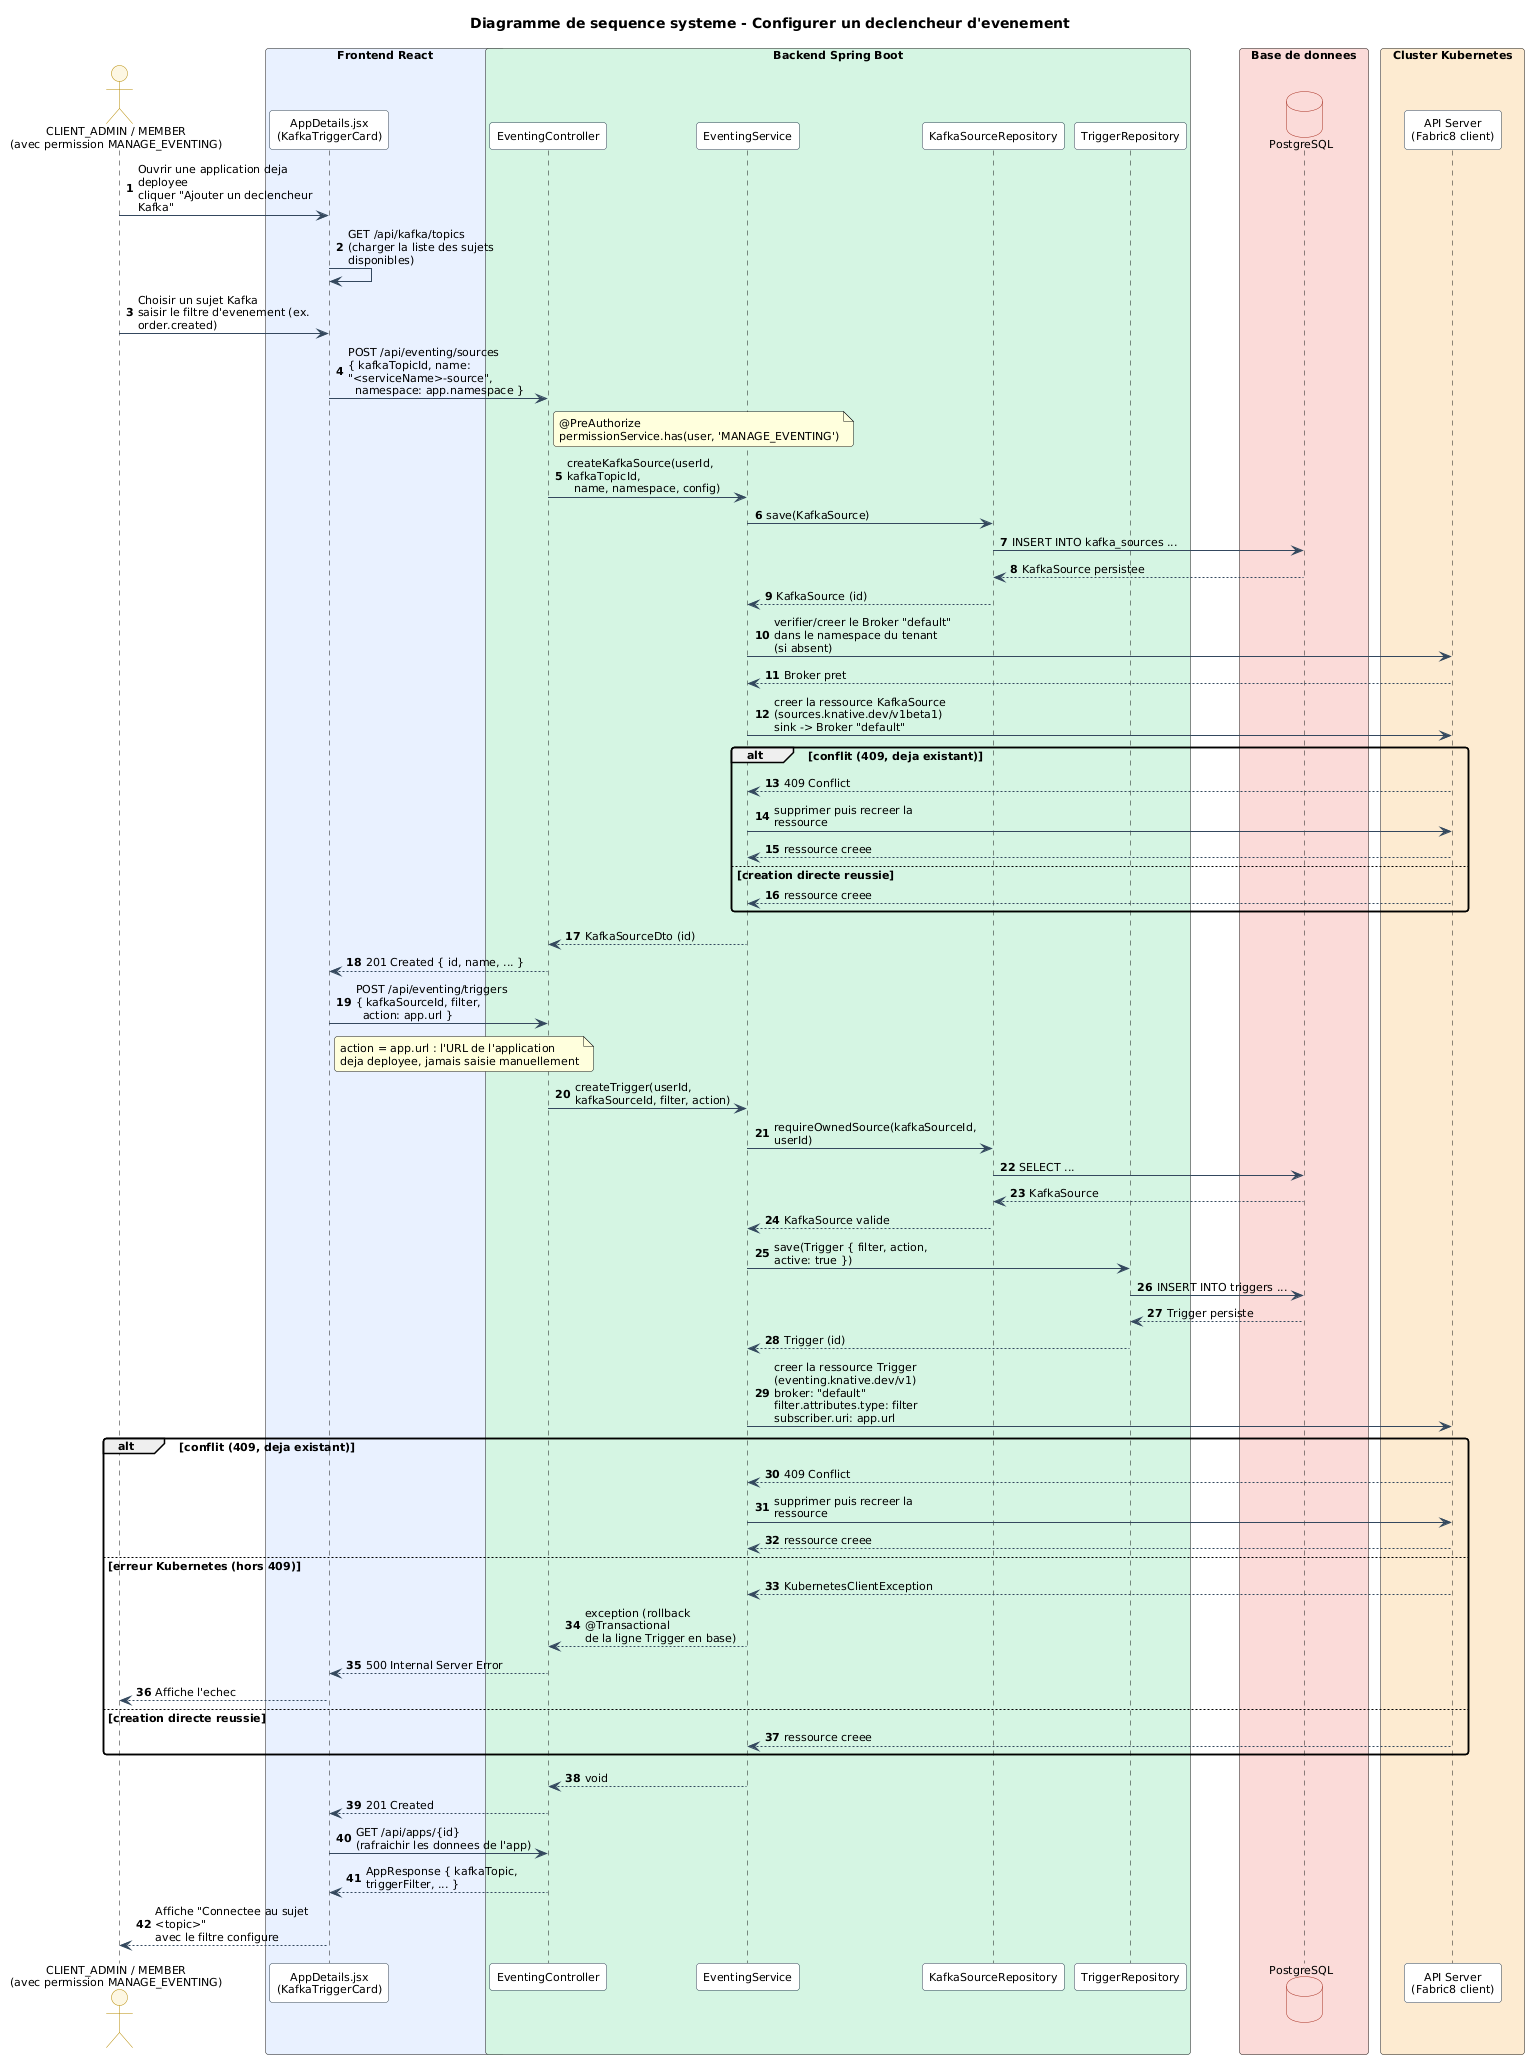
\includegraphics[width=\textwidth,height=0.85\textheight,keepaspectratio]{image/seq-eventing-trigger.png}
    \caption{Diagramme de séquence — Configurer un déclencheur d'événement}
    \label{fig:seq-eventing-trigger}
\end{figure}

\subsection{Réalisation du Sprint 5}

Fonctionnalité : Créer et gérer des sujets Kafka. La page de gestion Kafka du portail permet de créer, lister et supprimer les sujets du compte.

\begin{figure}[H]
 \centering
    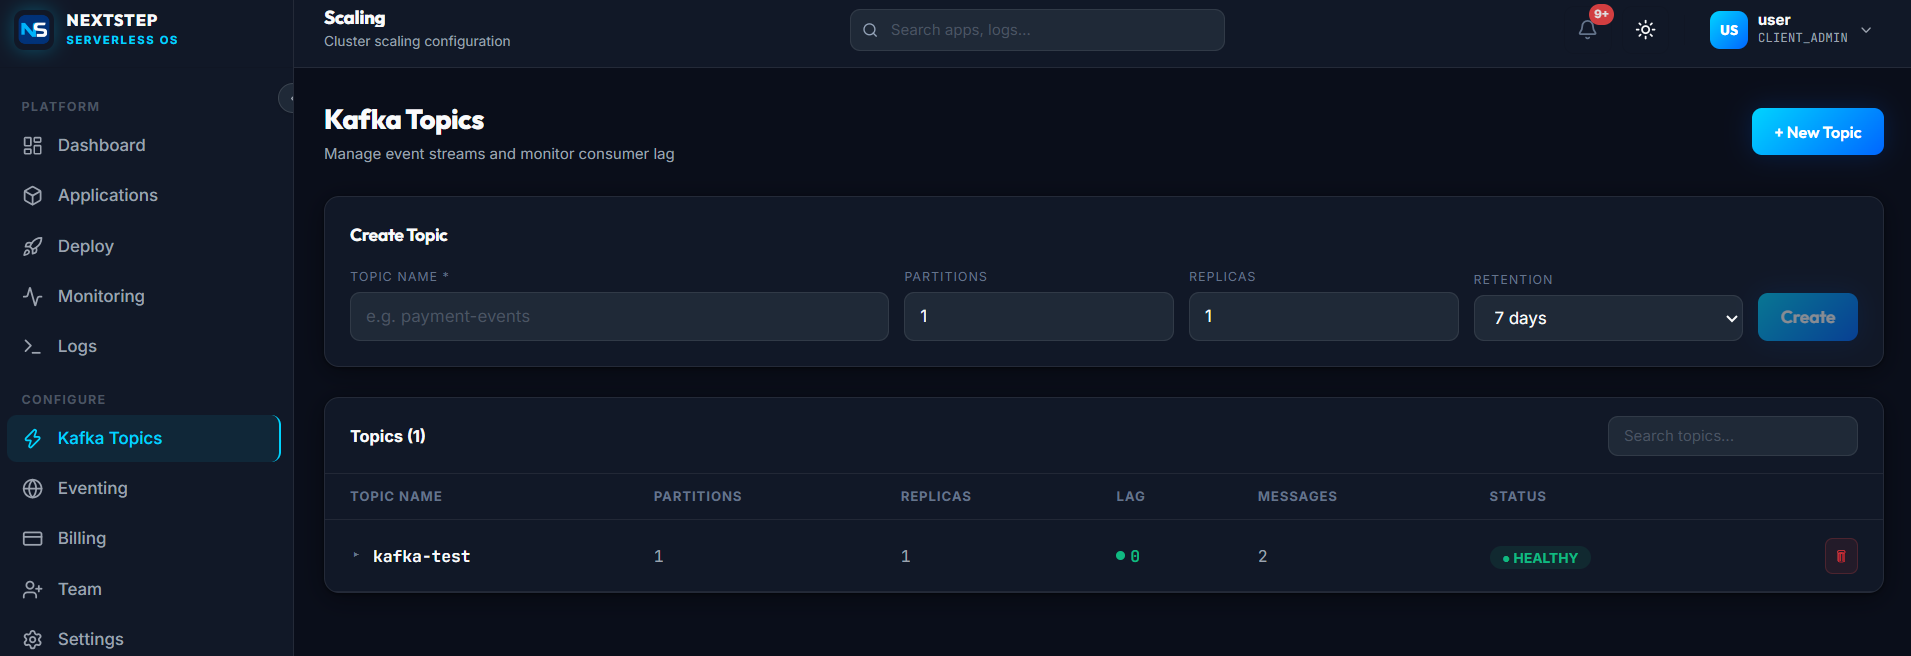
\includegraphics[width=0.9\textwidth]{image/Interface de gestion des sujets Kafka.png}
    \caption{Interface de gestion des sujets Kafka}
    \label{fig:capture-kafkatopics}
\end{figure}



Les trois ressources techniques que ce déclencheur assemble (Broker, KafkaSource, Trigger) sont visibles directement sur le cluster. La figure~\ref{fig:capture-eventing-broker} montre le Broker du tenant, à l'état prêt.

\begin{figure}[H]
 \centering
    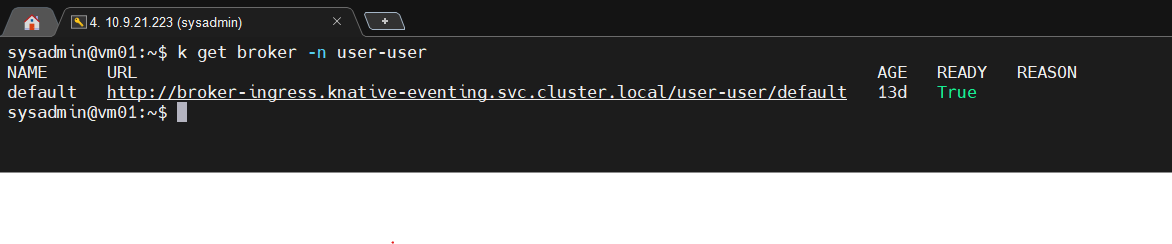
\includegraphics[width=0.92\textwidth]{image/capture_eventing_broker.png}
    \caption{Broker Knative Eventing du tenant}
    \label{fig:capture-eventing-broker}
\end{figure}

La figure~\ref{fig:capture-eventing-trigger} liste le Trigger créé pour une application : il référence le Broker et pointe vers l'URL du service cible.

\begin{figure}[H]
 \centering
    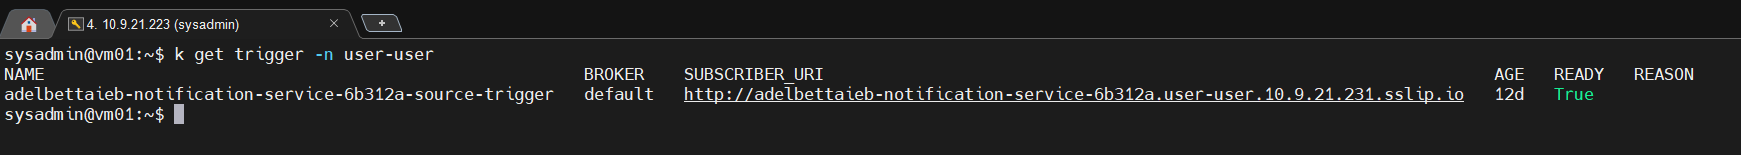
\includegraphics[width=0.92\textwidth]{image/capture_eventing_trigger.png}
    \caption{Trigger Knative Eventing associé à une application}
    \label{fig:capture-eventing-trigger}
\end{figure}

La figure~\ref{fig:capture-eventing-kafkasource} affiche la KafkaSource correspondante, qui consomme le sujet via le service de bootstrap du cluster Kafka.

\begin{figure}[H]
 \centering
    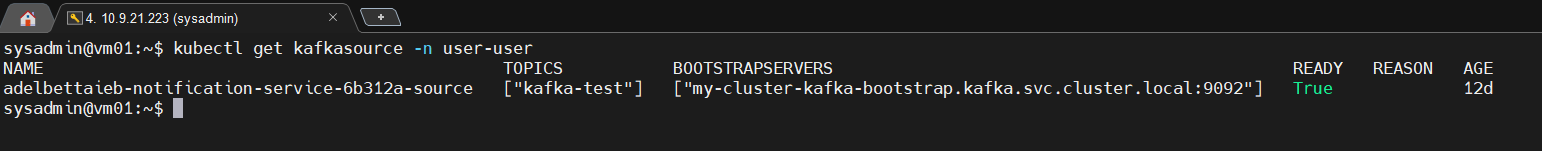
\includegraphics[width=0.92\textwidth]{image/capture_eventing_kafkasource.png}
    \caption{KafkaSource Knative Eventing associée au sujet Kafka}
    \label{fig:capture-eventing-kafkasource}
\end{figure}

Fonctionnalité : Publier un événement. Un CLIENT\_ADMIN ou un MEMBER publie un événement directement sur un sujet.

\begin{figure}[H]
 \centering
    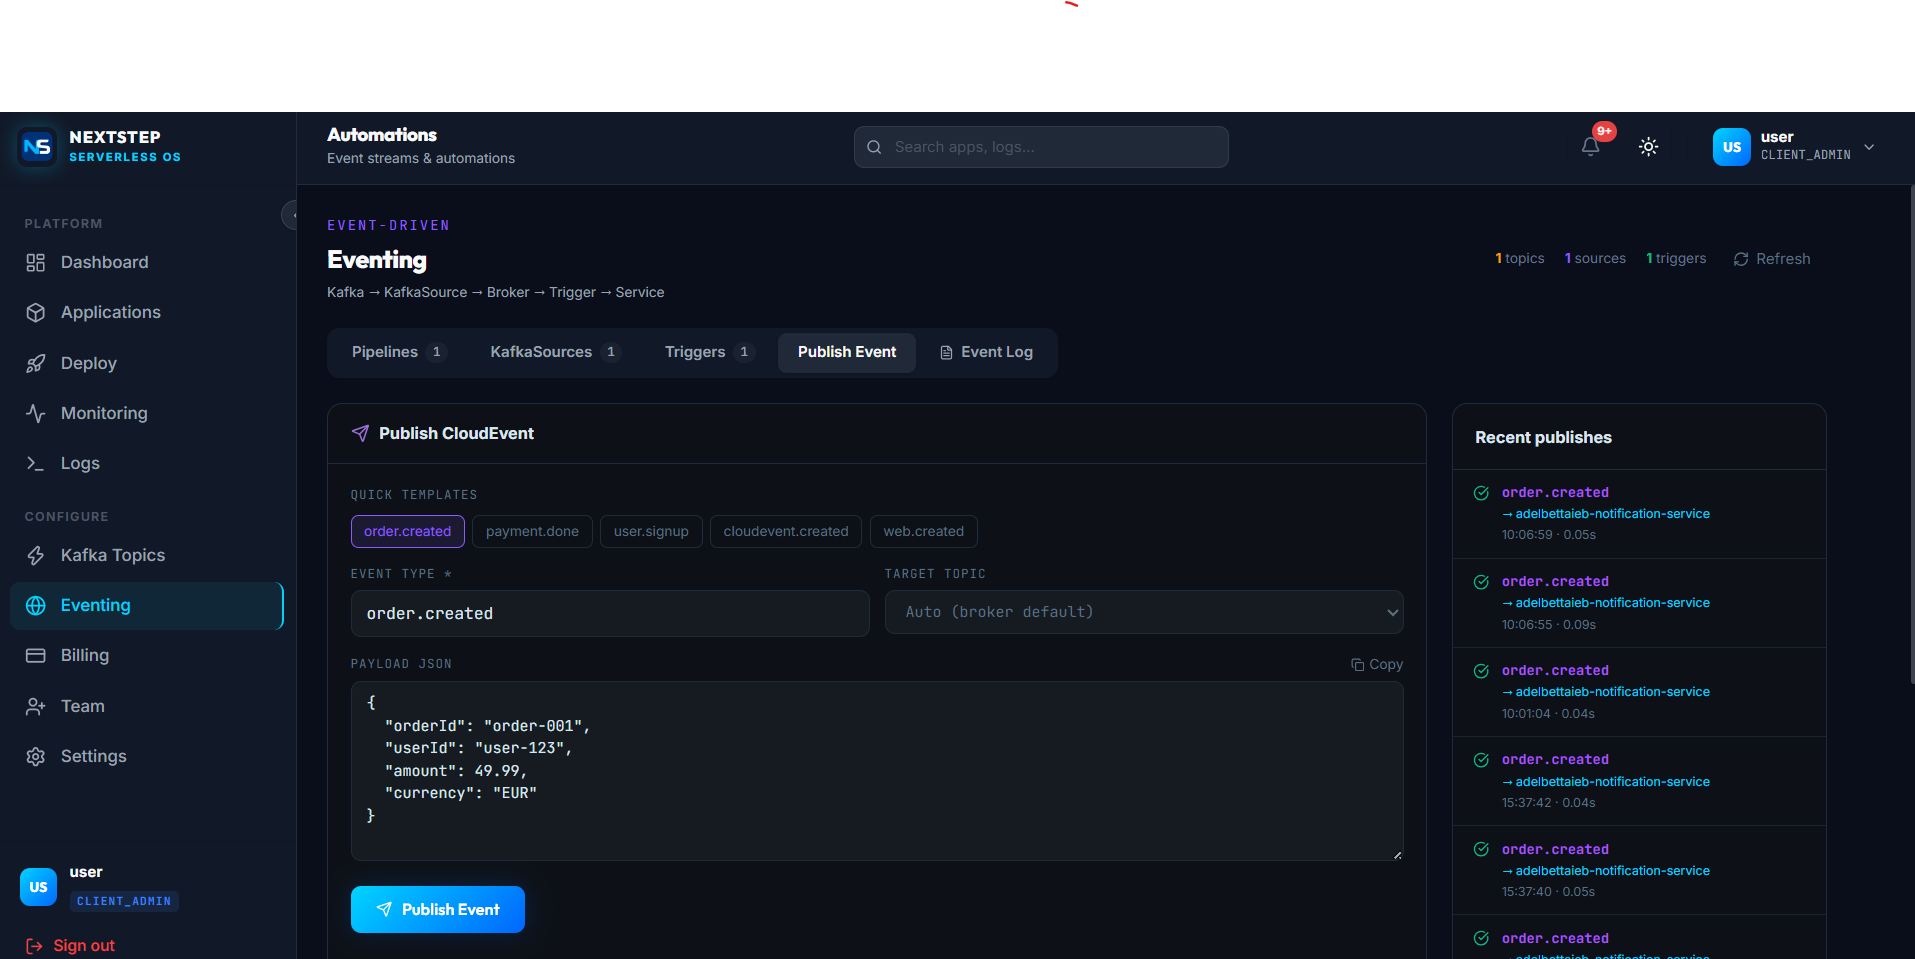
\includegraphics[width=0.9\textwidth]{image/Publication d’un événement.png}
    \caption{Publication d'un événement}
    \label{fig:capture-publish}
\end{figure}

Fonctionnalité : Vue globale et suppression forcée (ADMIN). L'ADMIN consulte, depuis la console d'administration, l'ensemble des sujets, sources et déclencheurs de tous les clients, et peut supprimer un sujet de force.

\begin{figure}[H]
 \centering
    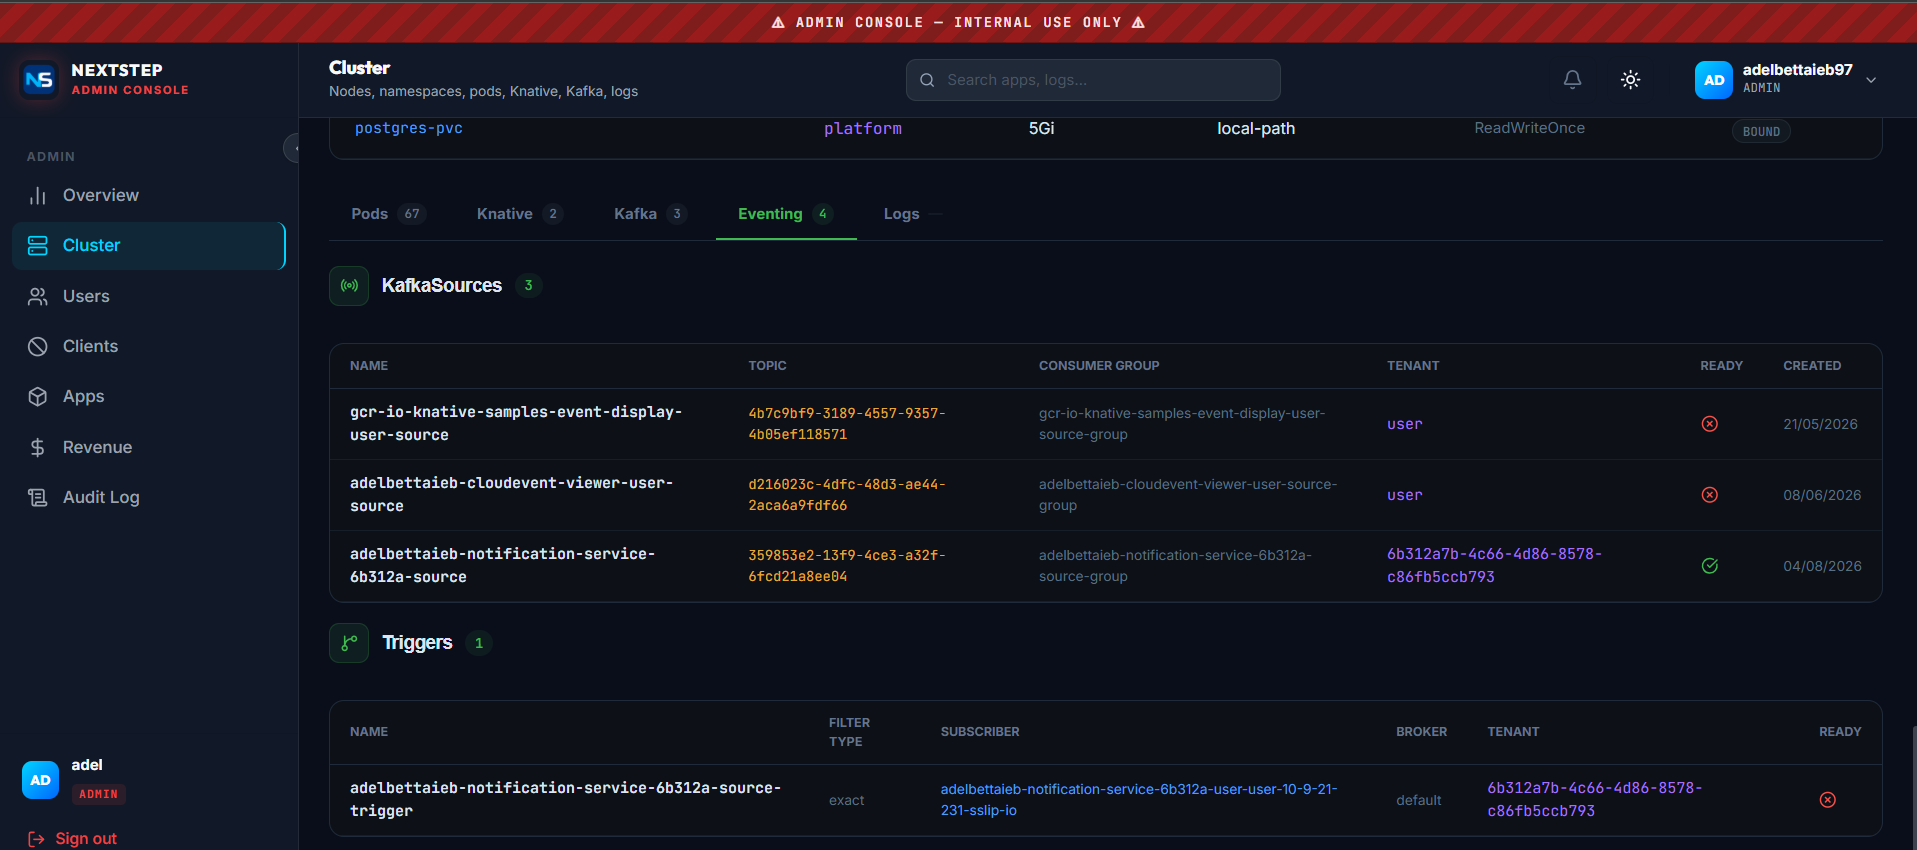
\includegraphics[width=0.9\textwidth]{image/ue administrateur des sujets, sources et déclencheurs.png}
    \caption{Vue administrateur des sujets, sources et déclencheurs}
    \label{fig:capture-admineventing}
\end{figure}

Le déploiement d'une application (Sprint 4) peut également câbler automatiquement un déclencheur, dans le même mouvement que la création de l'application, si le formulaire de déploiement renseigne un sujet Kafka.

\subsection{Conclusion}

Ce sprint relie Kafka et Knative Eventing en un service de messagerie événementielle complet et exposé au client : sujets, sources et déclencheurs sont créés, consultés et supprimés depuis le portail, avec une supervision globale côté ADMIN. La plateforme dispose désormais des trois grandes fonctions applicatives — accès, applications, événements — sur lesquelles s'appuie l'observabilité, objet du sprint suivant.

\clearpage
\section{Sprint 6 : Gestion de l'observabilité applicative}

\subsection{Introduction}

Ce sprint dote le portail client des capacités d'observation de ses propres applications : journaux de déploiement et applicatifs en temps réel, métriques de charge. La supervision de l'ensemble du cluster, réservée à l'ADMIN, est un domaine distinct traité au Sprint 9.

\subsection{Sprint Backlog}

Le tableau~\ref{tab:sb-sprint6} présente le backlog détaillé du Sprint 6, obtenu en décomposant chaque User Story retenue en tâches techniques.

\needspace{0.9\textheight}
{
\setlength{\LTleft}{-1.5cm}
\setlength{\LTright}{-1.5cm}
\setlength{\tabcolsep}{8pt}
\renewcommand{\arraystretch}{1.9}
\begin{longtable}{|p{6.6cm}|>{\raggedright\arraybackslash}p{8.1cm}|>{\centering\arraybackslash}p{2.3cm}|}
\hline
User Story & Tâches & Estimation \\
\hline
\endfirsthead
\hline
User Story & Tâches & Estimation \\
\hline
\endhead
\hline
\endfoot

\caption{Backlog du Sprint 6}
\label{tab:sb-sprint6}
\endlastfoot

\multirow{3}{6.6cm}{\centering En tant que CLIENT\_ADMIN, je veux consulter les journaux de déploiement de mes applications afin de diagnostiquer un problème.}
& Développer la consultation des journaux de déploiement. & 1 \\ \cline{2-3}
& Développer le filtrage par niveau. & 1 \\ \cline{2-3}
& Développer la page de consultation des journaux. & 1 \\ \hline

\multirow{2}{6.6cm}{\centering En tant que CLIENT\_ADMIN, je veux suivre les journaux applicatifs en temps réel afin d'observer le comportement de mon application en direct.}
& Développer le flux temps réel des journaux de déploiement. & 1 \\ \cline{2-3}
& Développer le flux temps réel des journaux bruts du conteneur. & 1 \\ \hline

\multirow{3}{6.6cm}{\centering En tant que CLIENT\_ADMIN, je veux consulter les métriques de mes applications afin d'évaluer leur charge et leurs performances.}
& Développer les métriques par application. & 1 \\ \cline{2-3}
& Développer le flux temps réel des métriques. & 1 \\ \cline{2-3}
& Développer la page de monitoring. & 1 \\ \hline

\multirow{2}{6.6cm}{\centering En tant qu'ADMIN, je veux consulter les journaux de déploiement de tous les locataires afin de superviser la plateforme.}
& Développer la vue administrateur des journaux. & 1 \\ \cline{2-3}
& Tester l'accès transversal aux journaux. & 1 \\ \hline

\end{longtable}
}

\subsection{Diagramme de cas d'utilisation du Sprint 6}

Le diagramme réunit CLIENT\_ADMIN et MEMBER (sous permission \texttt{VIEW\_LOGS}/\texttt{VIEW\_MONITORING}) et ADMIN, avec l'ensemble des fonctionnalités du sprint.

\begin{figure}[H]
 \centering
    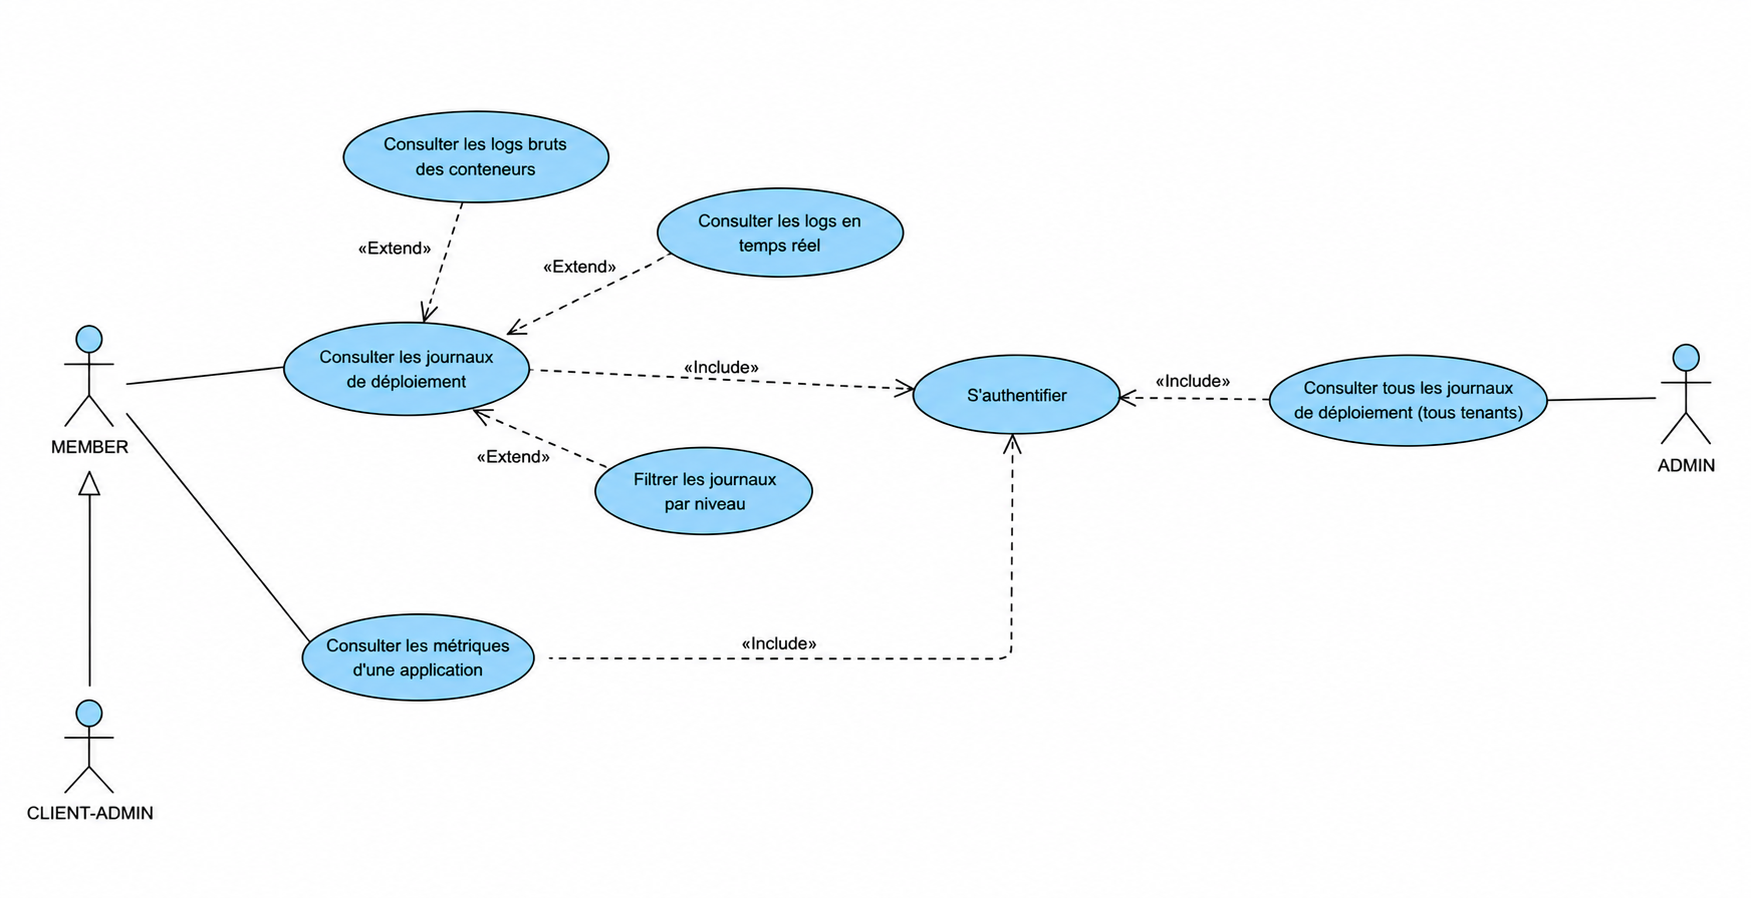
\includegraphics[width=\textwidth]{image/uc-sprint6.png}
    \caption{Diagramme de cas d'utilisation du Sprint 6 — Gestion de l'observabilité applicative}
    \label{fig:uc-sprint6}
\end{figure}

\subsection{Services Web}

\needspace{5cm}
\begin{longtable}{|p{6cm}|p{9.3cm}|}
\hline
Service Web & Description \\
\hline
\endfirsthead
\hline
Service Web & Description \\
\hline
\endhead
\hline
\endfoot
\endlastfoot
\texttt{GET /api/logs/apps/\{id\}} & Journaux de déploiement d'une application, filtrables par niveau. \\ \hline
\texttt{GET /api/logs/me} & Ses propres journaux. \\ \hline
\texttt{GET /api/logs/stream} (SSE) & Flux temps réel des journaux de déploiement. \\ \hline
\texttt{GET /api/logs/apps/\{id\}/pod-logs/stream} (SSE) & Flux temps réel des journaux bruts du conteneur. \\ \hline
\texttt{GET /api/metrics/apps/\{id\}} & Métriques d'une application (requêtes/s, latence, CPU, mémoire). \\ \hline
\texttt{GET /api/metrics/apps/\{id\}/stream} (SSE) & Flux temps réel des métriques d'une application. \\ \hline
\texttt{GET /api/admin/logs} & Journaux de déploiement de tous les locataires (ADMIN). \\ \hline
\end{longtable}

\subsection{Conception}

Deux fonctionnalités sont détaillées : la consultation des journaux en temps réel, dont la mise en œuvre a nécessité une correction de sécurité notable ; la consultation des métriques, appuyée sur Prometheus.

\subsubsection{Cas d'utilisation : « Consulter les journaux en temps réel »}

\subsubsection*{Description textuelle}

\renewcommand{\arraystretch}{1.5}
\begin{longtable}{|p{4cm}|p{11cm}|}
\hline
Nom & Consulter les journaux d'une application en temps réel \\
\hline
Acteur & CLIENT\_ADMIN, MEMBER (avec permission de consultation des journaux) \\
\hline
Pré-condition & L'application appartient au compte de l'utilisateur (ou de son CLIENT\_ADMIN) \\
\hline
Scénario nominal & 1. L'utilisateur ouvre la page de journaux de son application. 2. Le portail établit une connexion en flux continu vers le backend. 3. Le backend récupère les journaux du conteneur applicatif du pod concerné et les diffuse en temps réel. 4. L'utilisateur visualise les journaux au fil de leur émission. \\
\hline
Post-condition & L'utilisateur dispose d'une vue à jour de l'activité de son application. \\
\hline
\caption{Description textuelle du cas d'utilisation « Consulter les journaux en temps réel »}
\label{tab:uc-logs}
\end{longtable}

\subsubsection*{Diagramme de séquence}

\begin{figure}[H]
 \centering
    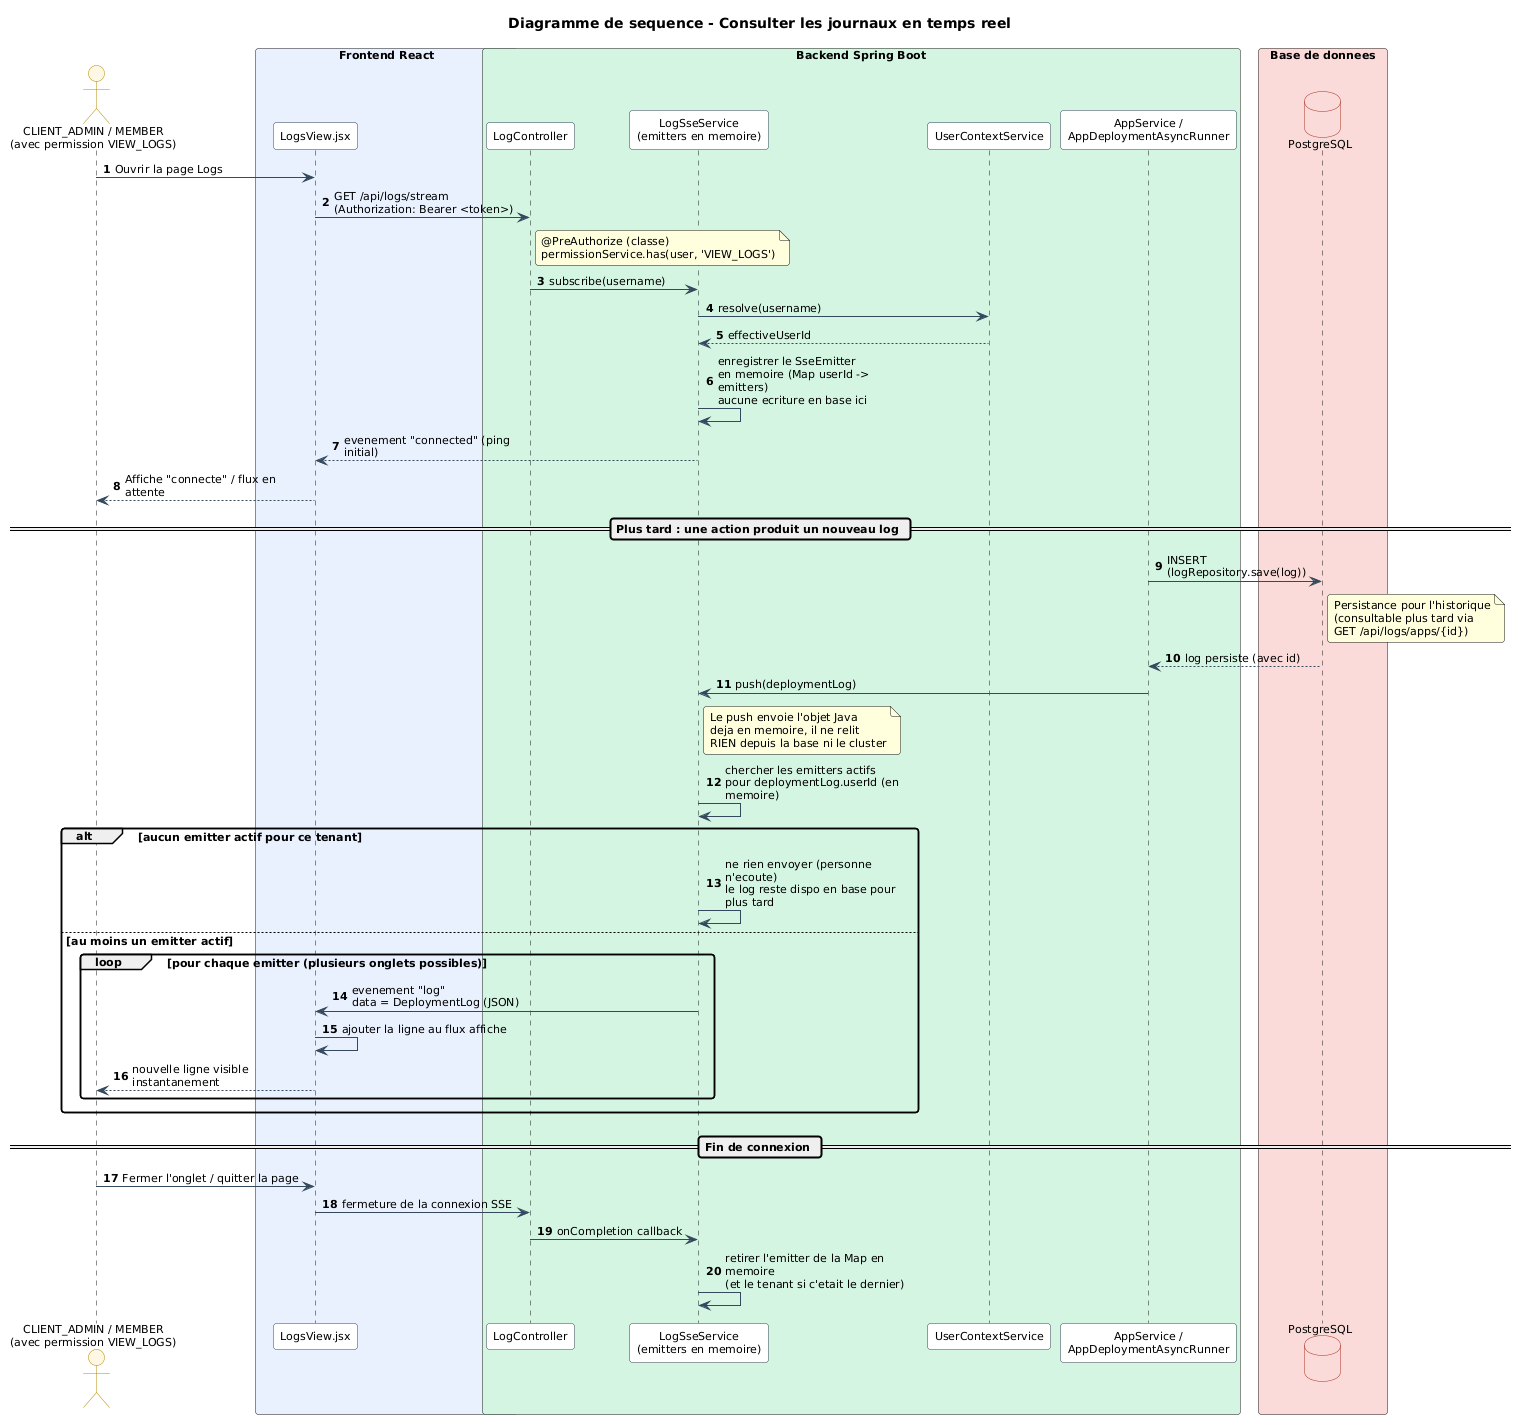
\includegraphics[width=\textwidth,height=0.85\textheight,keepaspectratio]{image/seq-logs.png}
    \caption{Diagramme de séquence — Consulter les journaux en temps réel}
    \label{fig:seq-logs}
\end{figure}



\subsection{Réalisation du Sprint 6}

Fonctionnalité : Consulter les journaux de déploiement. La page de journaux affiche, pour une application donnée, ses journaux de déploiement filtrables par niveau.

\begin{figure}[H]
 \centering
    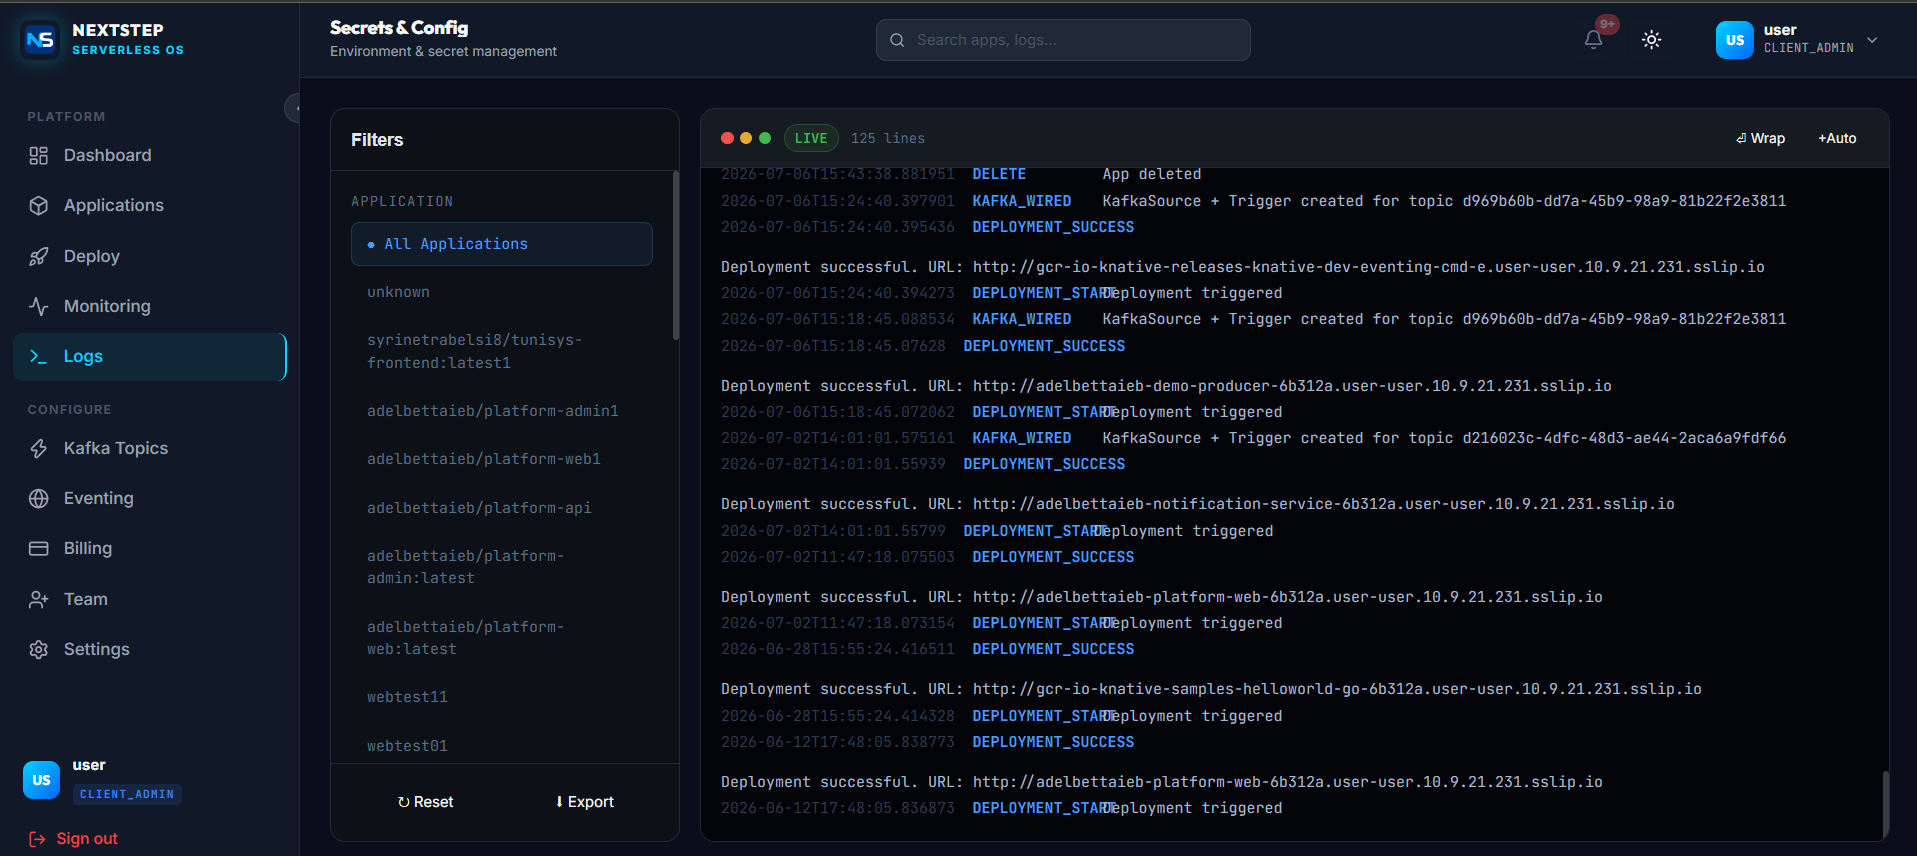
\includegraphics[width=0.9\textwidth]{image/Interface de consultation des journaux de déploiemen.png}
    \caption{Interface de consultation des journaux de déploiement}
    \label{fig:capture-deploylogs}
\end{figure}

Fonctionnalité : Suivre les journaux en temps réel. La même page diffuse en continu les journaux applicatifs bruts du conteneur.

\begin{figure}[H]
 \centering
    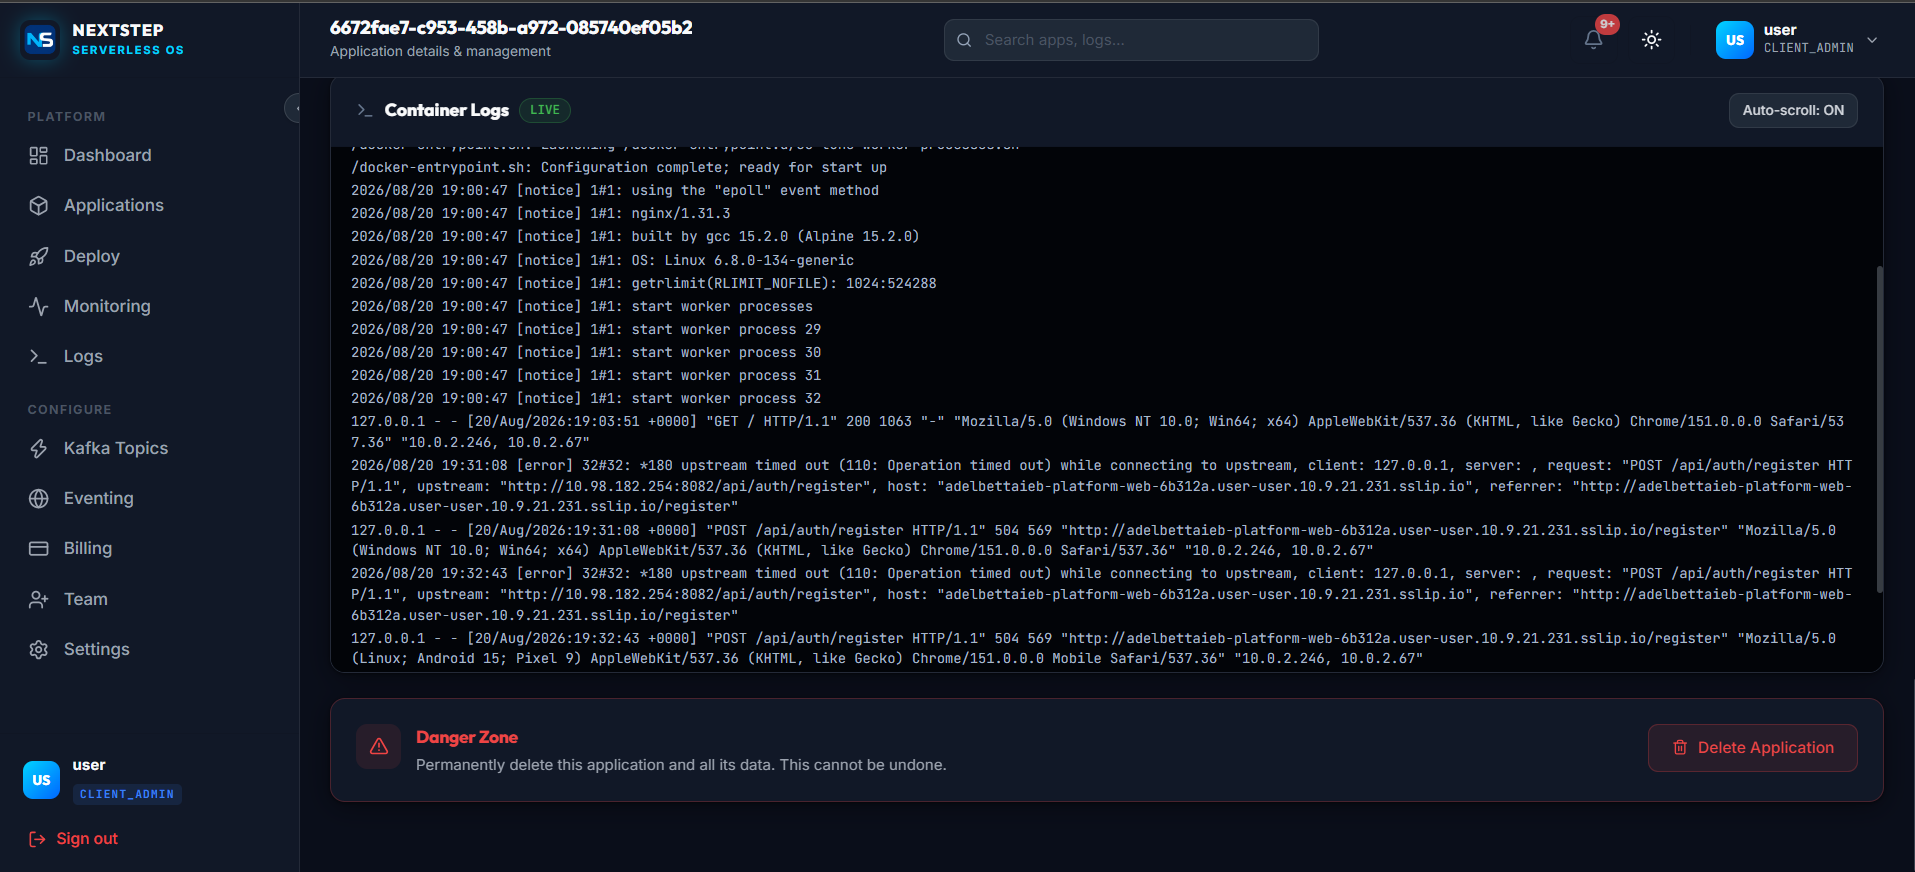
\includegraphics[width=0.9\textwidth]{image/Flux temps réel des journaux applicatifs.png}
    \caption{Flux temps réel des journaux applicatifs}
    \label{fig:capture-livelogs}
\end{figure}



Fonctionnalité : Consulter les journaux de tous les locataires (ADMIN). L'ADMIN consulte, depuis la console d'administration, les journaux de déploiement de l'ensemble des clients.

\begin{figure}[H]
 \centering
    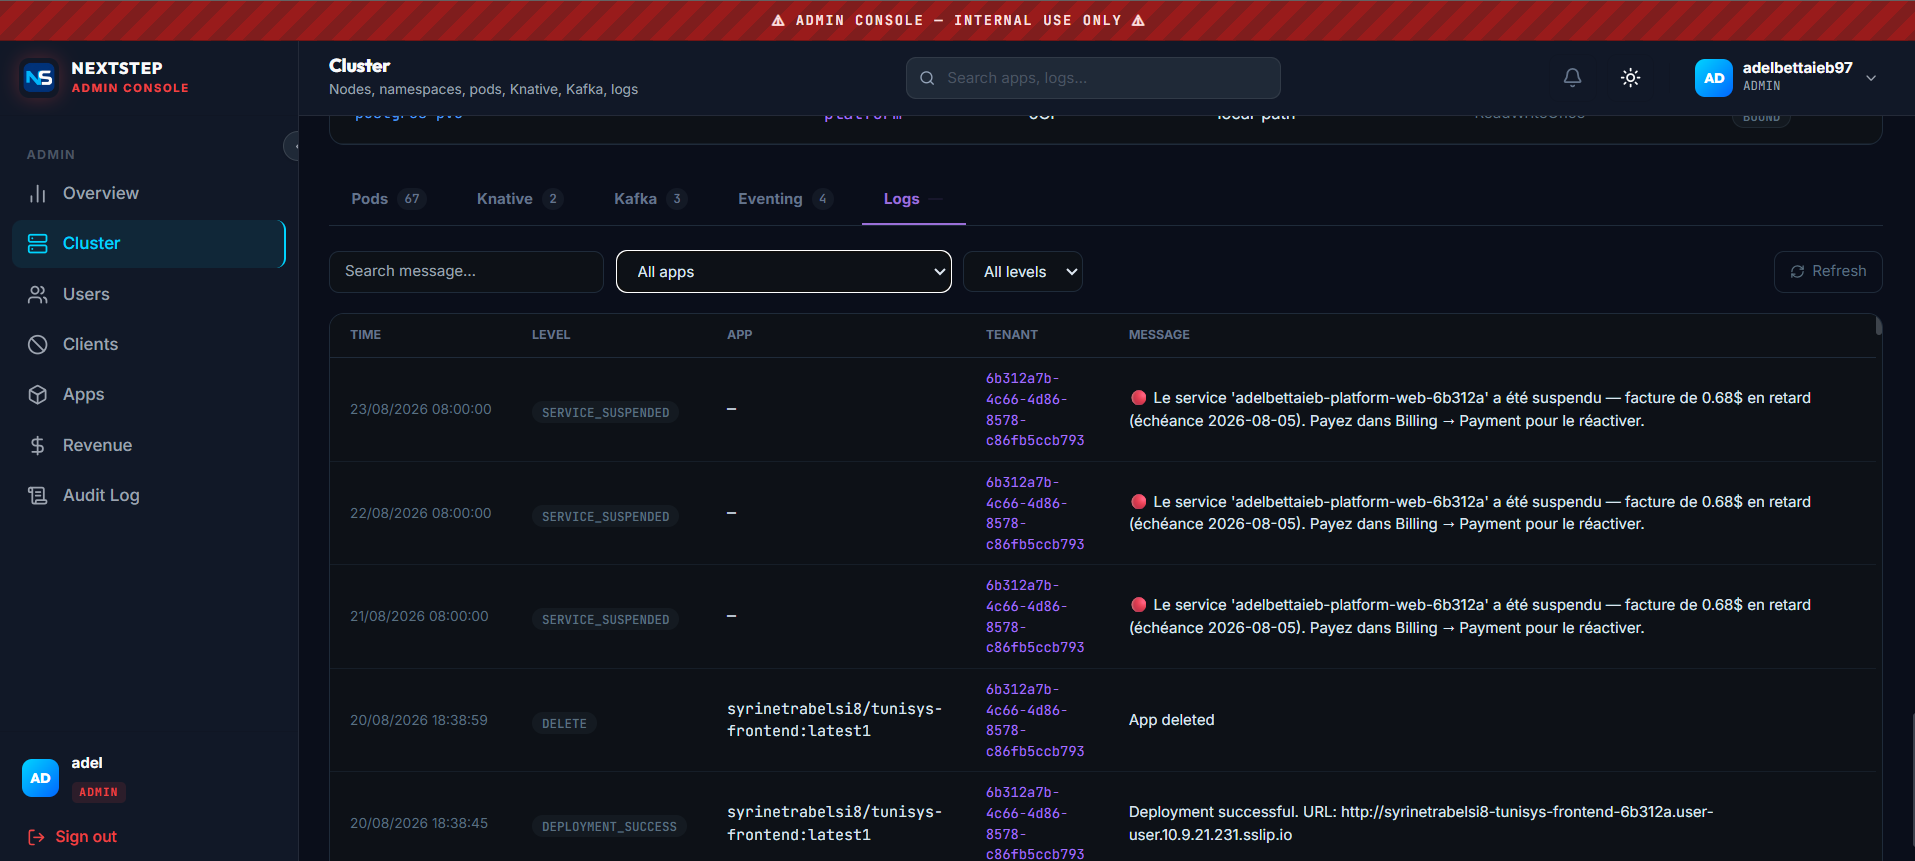
\includegraphics[width=0.9\textwidth]{image/Vue administrateur des journau.png}
    \caption{Vue administrateur des journaux}
    \label{fig:capture-adminlogs}
\end{figure}

\subsection{Conclusion}

Ce sprint livre l'observabilité applicative côté client : journaux et métriques, en différé comme en temps réel, avec une vue transversale côté ADMIN. La Release 1 est désormais complète : accès, applications, messagerie événementielle et observabilité constituent le cœur applicatif de la plateforme.

\section{Conclusion}

La Release 1 a transformé le socle technique de la Release 0 en un cœur applicatif cohérent, organisé par domaine de gestion plutôt que par brique livrée : accès et identité, cycle de vie des applications, messagerie événementielle, observabilité. Chaque sprint réunit tous les acteurs concernés par son domaine, du visiteur à l'ADMIN, et livre conjointement la brique backend et l'écran du portail qui l'expose. Plusieurs anomalies de cohérence et de sécurité identifiées au fil de ces sprints sont assumées comme limites du projet.
